\documentclass[twoside]{book}

% Packages required by doxygen
\usepackage{fixltx2e}
\usepackage{calc}
\usepackage{doxygen}
\usepackage[export]{adjustbox} % also loads graphicx
\usepackage{graphicx}
\usepackage[utf8]{inputenc}
\usepackage{makeidx}
\usepackage{multicol}
\usepackage{multirow}
\PassOptionsToPackage{warn}{textcomp}
\usepackage{textcomp}
\usepackage[nointegrals]{wasysym}
\usepackage[table]{xcolor}

% Font selection
\usepackage[T1]{fontenc}
\usepackage[scaled=.90]{helvet}
\usepackage{courier}
\usepackage{amssymb}
\usepackage{sectsty}
\renewcommand{\familydefault}{\sfdefault}
\allsectionsfont{%
  \fontseries{bc}\selectfont%
  \color{darkgray}%
}
\renewcommand{\DoxyLabelFont}{%
  \fontseries{bc}\selectfont%
  \color{darkgray}%
}
\newcommand{\+}{\discretionary{\mbox{\scriptsize$\hookleftarrow$}}{}{}}

% Page & text layout
\usepackage{geometry}
\geometry{%
  a4paper,%
  top=2.5cm,%
  bottom=2.5cm,%
  left=2.5cm,%
  right=2.5cm%
}
\tolerance=750
\hfuzz=15pt
\hbadness=750
\setlength{\emergencystretch}{15pt}
\setlength{\parindent}{0cm}
\setlength{\parskip}{3ex plus 2ex minus 2ex}
\makeatletter
\renewcommand{\paragraph}{%
  \@startsection{paragraph}{4}{0ex}{-1.0ex}{1.0ex}{%
    \normalfont\normalsize\bfseries\SS@parafont%
  }%
}
\renewcommand{\subparagraph}{%
  \@startsection{subparagraph}{5}{0ex}{-1.0ex}{1.0ex}{%
    \normalfont\normalsize\bfseries\SS@subparafont%
  }%
}
\makeatother

% Headers & footers
\usepackage{fancyhdr}
\pagestyle{fancyplain}
\fancyhead[LE]{\fancyplain{}{\bfseries\thepage}}
\fancyhead[CE]{\fancyplain{}{}}
\fancyhead[RE]{\fancyplain{}{\bfseries\leftmark}}
\fancyhead[LO]{\fancyplain{}{\bfseries\rightmark}}
\fancyhead[CO]{\fancyplain{}{}}
\fancyhead[RO]{\fancyplain{}{\bfseries\thepage}}
\fancyfoot[LE]{\fancyplain{}{}}
\fancyfoot[CE]{\fancyplain{}{}}
\fancyfoot[RE]{\fancyplain{}{\bfseries\scriptsize Generated by Doxygen }}
\fancyfoot[LO]{\fancyplain{}{\bfseries\scriptsize Generated by Doxygen }}
\fancyfoot[CO]{\fancyplain{}{}}
\fancyfoot[RO]{\fancyplain{}{}}
\renewcommand{\footrulewidth}{0.4pt}
\renewcommand{\chaptermark}[1]{%
  \markboth{#1}{}%
}
\renewcommand{\sectionmark}[1]{%
  \markright{\thesection\ #1}%
}

% Indices & bibliography
\usepackage{natbib}
\usepackage[titles]{tocloft}
\setcounter{tocdepth}{3}
\setcounter{secnumdepth}{5}
\makeindex

% Hyperlinks (required, but should be loaded last)
\usepackage{ifpdf}
\ifpdf
  \usepackage[pdftex,pagebackref=true]{hyperref}
\else
  \usepackage[ps2pdf,pagebackref=true]{hyperref}
\fi
\hypersetup{%
  colorlinks=true,%
  linkcolor=blue,%
  citecolor=blue,%
  unicode%
}

% Custom commands
\newcommand{\clearemptydoublepage}{%
  \newpage{\pagestyle{empty}\cleardoublepage}%
}

\usepackage{caption}
\captionsetup{labelsep=space,justification=centering,font={bf},singlelinecheck=off,skip=4pt,position=top}

%===== C O N T E N T S =====

\begin{document}

% Titlepage & ToC
\hypersetup{pageanchor=false,
             bookmarksnumbered=true,
             pdfencoding=unicode
            }
\pagenumbering{alph}
\begin{titlepage}
\vspace*{7cm}
\begin{center}%
{\Large Hassel\+Free\+Logger }\\
\vspace*{1cm}
{\large Generated by Doxygen 1.8.14}\\
\end{center}
\end{titlepage}
\clearemptydoublepage
\pagenumbering{roman}
\tableofcontents
\clearemptydoublepage
\pagenumbering{arabic}
\hypersetup{pageanchor=true}

%--- Begin generated contents ---
\chapter{Namespace Index}
\section{Packages}
Here are the packages with brief descriptions (if available)\+:\begin{DoxyCompactList}
\item\contentsline{section}{\mbox{\hyperlink{namespacenet}{net}} }{\pageref{namespacenet}}{}
\item\contentsline{section}{\mbox{\hyperlink{namespacenet_1_1dlinkddns}{net.\+dlinkddns}} }{\pageref{namespacenet_1_1dlinkddns}}{}
\item\contentsline{section}{\mbox{\hyperlink{namespacenet_1_1dlinkddns_1_1atulsaurabh}{net.\+dlinkddns.\+atulsaurabh}} }{\pageref{namespacenet_1_1dlinkddns_1_1atulsaurabh}}{}
\item\contentsline{section}{\mbox{\hyperlink{namespacenet_1_1dlinkddns_1_1atulsaurabh_1_1hasselfreelogger}{net.\+dlinkddns.\+atulsaurabh.\+hasselfreelogger}} }{\pageref{namespacenet_1_1dlinkddns_1_1atulsaurabh_1_1hasselfreelogger}}{}
\item\contentsline{section}{\mbox{\hyperlink{namespacenet_1_1dlinkddns_1_1atulsaurabh_1_1hasselfreelogger_1_1api}{net.\+dlinkddns.\+atulsaurabh.\+hasselfreelogger.\+api}} }{\pageref{namespacenet_1_1dlinkddns_1_1atulsaurabh_1_1hasselfreelogger_1_1api}}{}
\item\contentsline{section}{\mbox{\hyperlink{namespacenet_1_1dlinkddns_1_1atulsaurabh_1_1hasselfreelogger_1_1impl}{net.\+dlinkddns.\+atulsaurabh.\+hasselfreelogger.\+impl}} }{\pageref{namespacenet_1_1dlinkddns_1_1atulsaurabh_1_1hasselfreelogger_1_1impl}}{}
\end{DoxyCompactList}

\chapter{Hierarchical Index}
\section{Class Hierarchy}
This inheritance list is sorted roughly, but not completely, alphabetically\+:\begin{DoxyCompactList}
\item \contentsline{section}{net.\+dlinkddns.\+atulsaurabh.\+hasselfreelogger.\+api.\+Logger}{\pageref{interfacenet_1_1dlinkddns_1_1atulsaurabh_1_1hasselfreelogger_1_1api_1_1_logger}}{}
\begin{DoxyCompactList}
\item \contentsline{section}{net.\+dlinkddns.\+atulsaurabh.\+hasselfreelogger.\+impl.\+Hassel\+Free\+Logger}{\pageref{classnet_1_1dlinkddns_1_1atulsaurabh_1_1hasselfreelogger_1_1impl_1_1_hassel_free_logger}}{}
\end{DoxyCompactList}
\end{DoxyCompactList}

\chapter{Class Index}
\section{Class List}
Here are the classes, structs, unions and interfaces with brief descriptions\+:\begin{DoxyCompactList}
\item\contentsline{section}{\mbox{\hyperlink{classnet_1_1dlinkddns_1_1atulsaurabh_1_1hasselfreelogger_1_1impl_1_1_hassel_free_logger}{net.\+dlinkddns.\+atulsaurabh.\+hasselfreelogger.\+impl.\+Hassel\+Free\+Logger}} }{\pageref{classnet_1_1dlinkddns_1_1atulsaurabh_1_1hasselfreelogger_1_1impl_1_1_hassel_free_logger}}{}
\item\contentsline{section}{\mbox{\hyperlink{interfacenet_1_1dlinkddns_1_1atulsaurabh_1_1hasselfreelogger_1_1api_1_1_logger}{net.\+dlinkddns.\+atulsaurabh.\+hasselfreelogger.\+api.\+Logger}} }{\pageref{interfacenet_1_1dlinkddns_1_1atulsaurabh_1_1hasselfreelogger_1_1api_1_1_logger}}{}
\end{DoxyCompactList}

\chapter{File Index}
\section{File List}
Here is a list of all files with brief descriptions\+:\begin{DoxyCompactList}
\item\contentsline{section}{src/main/java/net/dlinkddns/atulsaurabh/hasselfreelogger/api/\mbox{\hyperlink{_logger_8java}{Logger.\+java}} }{\pageref{_logger_8java}}{}
\item\contentsline{section}{src/main/java/net/dlinkddns/atulsaurabh/hasselfreelogger/impl/\mbox{\hyperlink{_hassel_free_logger_8java}{Hassel\+Free\+Logger.\+java}} }{\pageref{_hassel_free_logger_8java}}{}
\end{DoxyCompactList}

\chapter{Namespace Documentation}
\hypertarget{namespacenet}{}\section{Package net}
\label{namespacenet}\index{net@{net}}
\subsection*{Packages}
\begin{DoxyCompactItemize}
\item 
package \mbox{\hyperlink{namespacenet_1_1dlinkddns}{dlinkddns}}
\end{DoxyCompactItemize}

\hypertarget{namespacenet_1_1dlinkddns}{}\section{Package net.\+dlinkddns}
\label{namespacenet_1_1dlinkddns}\index{net.\+dlinkddns@{net.\+dlinkddns}}
\subsection*{Packages}
\begin{DoxyCompactItemize}
\item 
package \mbox{\hyperlink{namespacenet_1_1dlinkddns_1_1atulsaurabh}{atulsaurabh}}
\end{DoxyCompactItemize}

\hypertarget{namespacenet_1_1dlinkddns_1_1atulsaurabh}{}\section{Package net.\+dlinkddns.\+atulsaurabh}
\label{namespacenet_1_1dlinkddns_1_1atulsaurabh}\index{net.\+dlinkddns.\+atulsaurabh@{net.\+dlinkddns.\+atulsaurabh}}
\subsection*{Packages}
\begin{DoxyCompactItemize}
\item 
package \mbox{\hyperlink{namespacenet_1_1dlinkddns_1_1atulsaurabh_1_1hasselfreelogger}{hasselfreelogger}}
\end{DoxyCompactItemize}

\hypertarget{namespacenet_1_1dlinkddns_1_1atulsaurabh_1_1hasselfreelogger}{}\section{Package net.\+dlinkddns.\+atulsaurabh.\+hasselfreelogger}
\label{namespacenet_1_1dlinkddns_1_1atulsaurabh_1_1hasselfreelogger}\index{net.\+dlinkddns.\+atulsaurabh.\+hasselfreelogger@{net.\+dlinkddns.\+atulsaurabh.\+hasselfreelogger}}
\subsection*{Packages}
\begin{DoxyCompactItemize}
\item 
package \mbox{\hyperlink{namespacenet_1_1dlinkddns_1_1atulsaurabh_1_1hasselfreelogger_1_1api}{api}}
\item 
package \mbox{\hyperlink{namespacenet_1_1dlinkddns_1_1atulsaurabh_1_1hasselfreelogger_1_1impl}{impl}}
\end{DoxyCompactItemize}

\hypertarget{namespacenet_1_1dlinkddns_1_1atulsaurabh_1_1hasselfreelogger_1_1api}{}\section{Package net.\+dlinkddns.\+atulsaurabh.\+hasselfreelogger.\+api}
\label{namespacenet_1_1dlinkddns_1_1atulsaurabh_1_1hasselfreelogger_1_1api}\index{net.\+dlinkddns.\+atulsaurabh.\+hasselfreelogger.\+api@{net.\+dlinkddns.\+atulsaurabh.\+hasselfreelogger.\+api}}
\subsection*{Classes}
\begin{DoxyCompactItemize}
\item 
interface \mbox{\hyperlink{interfacenet_1_1dlinkddns_1_1atulsaurabh_1_1hasselfreelogger_1_1api_1_1_logger}{Logger}}
\end{DoxyCompactItemize}

\hypertarget{namespacenet_1_1dlinkddns_1_1atulsaurabh_1_1hasselfreelogger_1_1impl}{}\section{Package net.\+dlinkddns.\+atulsaurabh.\+hasselfreelogger.\+impl}
\label{namespacenet_1_1dlinkddns_1_1atulsaurabh_1_1hasselfreelogger_1_1impl}\index{net.\+dlinkddns.\+atulsaurabh.\+hasselfreelogger.\+impl@{net.\+dlinkddns.\+atulsaurabh.\+hasselfreelogger.\+impl}}
\subsection*{Classes}
\begin{DoxyCompactItemize}
\item 
class \mbox{\hyperlink{classnet_1_1dlinkddns_1_1atulsaurabh_1_1hasselfreelogger_1_1impl_1_1_hassel_free_logger}{Hassel\+Free\+Logger}}
\end{DoxyCompactItemize}

\chapter{Class Documentation}
\hypertarget{classnet_1_1dlinkddns_1_1atulsaurabh_1_1hasselfreelogger_1_1impl_1_1_hassel_free_logger}{}\section{net.\+dlinkddns.\+atulsaurabh.\+hasselfreelogger.\+impl.\+Hassel\+Free\+Logger Class Reference}
\label{classnet_1_1dlinkddns_1_1atulsaurabh_1_1hasselfreelogger_1_1impl_1_1_hassel_free_logger}\index{net.\+dlinkddns.\+atulsaurabh.\+hasselfreelogger.\+impl.\+Hassel\+Free\+Logger@{net.\+dlinkddns.\+atulsaurabh.\+hasselfreelogger.\+impl.\+Hassel\+Free\+Logger}}
Inheritance diagram for net.\+dlinkddns.\+atulsaurabh.\+hasselfreelogger.\+impl.\+Hassel\+Free\+Logger\+:\begin{figure}[H]
\begin{center}
\leavevmode
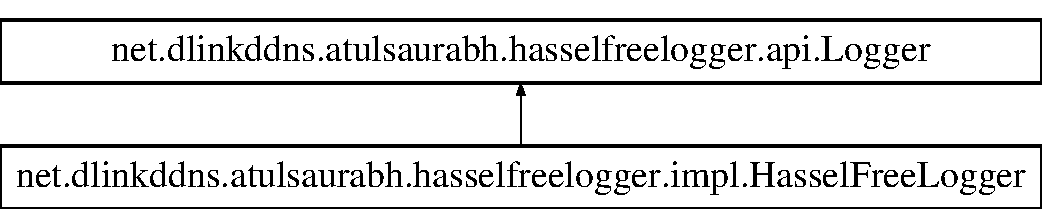
\includegraphics[height=2.000000cm]{d8/de1/classnet_1_1dlinkddns_1_1atulsaurabh_1_1hasselfreelogger_1_1impl_1_1_hassel_free_logger}
\end{center}
\end{figure}
\subsection*{Public Member Functions}
\begin{DoxyCompactItemize}
\item 
\mbox{\hyperlink{classnet_1_1dlinkddns_1_1atulsaurabh_1_1hasselfreelogger_1_1impl_1_1_hassel_free_logger_a603e83e38bc2c011dd3e5edf074acb1d}{Hassel\+Free\+Logger}} ()
\item 
\mbox{\hyperlink{classnet_1_1dlinkddns_1_1atulsaurabh_1_1hasselfreelogger_1_1impl_1_1_hassel_free_logger_a1210504fcaba4ae6c3283c0fc0882380}{Hassel\+Free\+Logger}} (Properties properties)
\item 
void \mbox{\hyperlink{classnet_1_1dlinkddns_1_1atulsaurabh_1_1hasselfreelogger_1_1impl_1_1_hassel_free_logger_a9dbc7356642960679aaa76cc054ce456}{set\+Configuration}} (Properties properties)
\item 
void \mbox{\hyperlink{classnet_1_1dlinkddns_1_1atulsaurabh_1_1hasselfreelogger_1_1impl_1_1_hassel_free_logger_a478d877ebdbb5cb2796ad23d0dafe369}{log\+Fatal}} (String message)
\item 
void \mbox{\hyperlink{classnet_1_1dlinkddns_1_1atulsaurabh_1_1hasselfreelogger_1_1impl_1_1_hassel_free_logger_a40d4e893854bc742145dbf2fe5d2aa43}{log\+Fatal}} (Class error\+Class, String message)
\item 
void \mbox{\hyperlink{classnet_1_1dlinkddns_1_1atulsaurabh_1_1hasselfreelogger_1_1impl_1_1_hassel_free_logger_a546bc74e8eec8333893e294a98bbe939}{log\+Fatal}} (Class error\+Class, String message, Throwable throwable)
\item 
void \mbox{\hyperlink{classnet_1_1dlinkddns_1_1atulsaurabh_1_1hasselfreelogger_1_1impl_1_1_hassel_free_logger_af433939b275c708e5334f56a6444e2af}{log\+All}} (String message)
\item 
void \mbox{\hyperlink{classnet_1_1dlinkddns_1_1atulsaurabh_1_1hasselfreelogger_1_1impl_1_1_hassel_free_logger_ade5a00300f3406a3a64ca003b1799dbd}{log\+All}} (Class error\+Class, String message)
\item 
void \mbox{\hyperlink{classnet_1_1dlinkddns_1_1atulsaurabh_1_1hasselfreelogger_1_1impl_1_1_hassel_free_logger_a6b63592b0c825713f2bc861b6d487df8}{log\+All}} (Class error\+Class, String message, Throwable throwable)
\item 
String \mbox{\hyperlink{classnet_1_1dlinkddns_1_1atulsaurabh_1_1hasselfreelogger_1_1impl_1_1_hassel_free_logger_a8309e8b9abe877ce11e6b04faf48e8c1}{get\+Conversion\+Pattern}} ()
\item 
void \mbox{\hyperlink{classnet_1_1dlinkddns_1_1atulsaurabh_1_1hasselfreelogger_1_1impl_1_1_hassel_free_logger_a23a1e3b5c56528e197c7eb3832e7c69e}{set\+Conversion\+Pattern}} (String \mbox{\hyperlink{classnet_1_1dlinkddns_1_1atulsaurabh_1_1hasselfreelogger_1_1impl_1_1_hassel_free_logger_a9e05fdd81d207cfd60132cc3b15b26cb}{conversion\+Pattern}})
\item 
void \mbox{\hyperlink{classnet_1_1dlinkddns_1_1atulsaurabh_1_1hasselfreelogger_1_1impl_1_1_hassel_free_logger_a9e847886284d6a0f7edef691e2d11efd}{log\+Warning}} (String message)
\item 
void \mbox{\hyperlink{classnet_1_1dlinkddns_1_1atulsaurabh_1_1hasselfreelogger_1_1impl_1_1_hassel_free_logger_ad5f8400bc0ea2500509a4154cfa48bf5}{log\+Warning}} (Class warning\+Class, String message)
\item 
void \mbox{\hyperlink{classnet_1_1dlinkddns_1_1atulsaurabh_1_1hasselfreelogger_1_1impl_1_1_hassel_free_logger_ac5e36ee2095f1f92c90885360a0fd1f1}{log\+Warning}} (Class warning\+Class, String message, Throwable throwable)
\item 
void \mbox{\hyperlink{classnet_1_1dlinkddns_1_1atulsaurabh_1_1hasselfreelogger_1_1impl_1_1_hassel_free_logger_abca8e8a8a8c85d582092b35fc395d726}{log\+Info}} (String message)
\item 
void \mbox{\hyperlink{classnet_1_1dlinkddns_1_1atulsaurabh_1_1hasselfreelogger_1_1impl_1_1_hassel_free_logger_a011e8791e13b815927a16254e9cfa2a3}{log\+Info}} (Class info\+Class, String message)
\item 
void \mbox{\hyperlink{classnet_1_1dlinkddns_1_1atulsaurabh_1_1hasselfreelogger_1_1impl_1_1_hassel_free_logger_ac0596a92805b29d9402a9eb17c71891a}{log\+Info}} (Class info\+Class, String message, Throwable throwable)
\item 
void \mbox{\hyperlink{classnet_1_1dlinkddns_1_1atulsaurabh_1_1hasselfreelogger_1_1impl_1_1_hassel_free_logger_a7aafa489bd14255cbdb43c1f2494d433}{log\+Debug}} (String message)
\item 
void \mbox{\hyperlink{classnet_1_1dlinkddns_1_1atulsaurabh_1_1hasselfreelogger_1_1impl_1_1_hassel_free_logger_a7c65f65791b715d7c72a2227a8a00bdc}{log\+Debug}} (Class debug\+Class, String message)
\item 
void \mbox{\hyperlink{classnet_1_1dlinkddns_1_1atulsaurabh_1_1hasselfreelogger_1_1impl_1_1_hassel_free_logger_a0995d59f7b5262af4be98f4e7ba21cd0}{log\+Debug}} (Class debug\+Class, String message, Throwable throwable)
\item 
void \mbox{\hyperlink{classnet_1_1dlinkddns_1_1atulsaurabh_1_1hasselfreelogger_1_1impl_1_1_hassel_free_logger_a94641af9c6c39ea601d5c41bf68a4b1f}{log\+Error}} (String message)
\item 
void \mbox{\hyperlink{classnet_1_1dlinkddns_1_1atulsaurabh_1_1hasselfreelogger_1_1impl_1_1_hassel_free_logger_a47870e52004c823f0ef365f5d41afd6b}{log\+Error}} (Class error\+Class, String message)
\item 
void \mbox{\hyperlink{classnet_1_1dlinkddns_1_1atulsaurabh_1_1hasselfreelogger_1_1impl_1_1_hassel_free_logger_acf886c01c94bba98b551f98e2ad8ce4f}{log\+Error}} (Class error\+Class, String message, Throwable throwable)
\item 
boolean \mbox{\hyperlink{classnet_1_1dlinkddns_1_1atulsaurabh_1_1hasselfreelogger_1_1impl_1_1_hassel_free_logger_a1264dcefa68828985aa843e545ff41b6}{is\+Rolling\+On}} ()
\item 
void \mbox{\hyperlink{classnet_1_1dlinkddns_1_1atulsaurabh_1_1hasselfreelogger_1_1impl_1_1_hassel_free_logger_a9ef8b4f7c9615f50c03f168f1b949f64}{set\+Rolling\+On}} (boolean \mbox{\hyperlink{classnet_1_1dlinkddns_1_1atulsaurabh_1_1hasselfreelogger_1_1impl_1_1_hassel_free_logger_a7d4b387ecfa16af11b2b169ac3f062a3}{rolling\+On}})
\item 
String \mbox{\hyperlink{classnet_1_1dlinkddns_1_1atulsaurabh_1_1hasselfreelogger_1_1impl_1_1_hassel_free_logger_a9b56e6059627b493e8f5ebff888795a0}{get\+Date\+Pattern}} ()
\item 
void \mbox{\hyperlink{classnet_1_1dlinkddns_1_1atulsaurabh_1_1hasselfreelogger_1_1impl_1_1_hassel_free_logger_a72529568d69eea543b2238a466cedf8d}{set\+Date\+Pattern}} (String \mbox{\hyperlink{classnet_1_1dlinkddns_1_1atulsaurabh_1_1hasselfreelogger_1_1impl_1_1_hassel_free_logger_aa2dcc355996a8d6e3cc52fad0774f0fd}{date\+Pattern}})
\end{DoxyCompactItemize}
\subsection*{Private Member Functions}
\begin{DoxyCompactItemize}
\item 
void \mbox{\hyperlink{classnet_1_1dlinkddns_1_1atulsaurabh_1_1hasselfreelogger_1_1impl_1_1_hassel_free_logger_af159818a248f7cd39c79ead6e08efda8}{set\+Options}} (Properties properties)
\item 
org.\+apache.\+log4j.\+Logger \mbox{\hyperlink{classnet_1_1dlinkddns_1_1atulsaurabh_1_1hasselfreelogger_1_1impl_1_1_hassel_free_logger_af0d3b51d857b4df4ef5f5356e2e07ada}{log}} (Class error\+Class, Level level)
\item 
Daily\+Rolling\+File\+Appender \mbox{\hyperlink{classnet_1_1dlinkddns_1_1atulsaurabh_1_1hasselfreelogger_1_1impl_1_1_hassel_free_logger_a33e52eaefee44a20c6146c29abf4fb3d}{get\+Rolling\+File\+Adapter}} (String file\+Name)  throws U\+R\+I\+Syntax\+Exception   
\end{DoxyCompactItemize}
\subsection*{Private Attributes}
\begin{DoxyCompactItemize}
\item 
String \mbox{\hyperlink{classnet_1_1dlinkddns_1_1atulsaurabh_1_1hasselfreelogger_1_1impl_1_1_hassel_free_logger_adbc3e4df8942c21a7328cd04a141bb34}{log\+\_\+directory\+\_\+name}}
\item 
String \mbox{\hyperlink{classnet_1_1dlinkddns_1_1atulsaurabh_1_1hasselfreelogger_1_1impl_1_1_hassel_free_logger_acd10249a6d38c569825ab0423eada5c6}{fatal\+\_\+log\+\_\+file\+\_\+name}}
\item 
String \mbox{\hyperlink{classnet_1_1dlinkddns_1_1atulsaurabh_1_1hasselfreelogger_1_1impl_1_1_hassel_free_logger_aca408fb67e695b6236ca9678fa45e88a}{debug\+\_\+log\+\_\+file\+\_\+name}}
\item 
String \mbox{\hyperlink{classnet_1_1dlinkddns_1_1atulsaurabh_1_1hasselfreelogger_1_1impl_1_1_hassel_free_logger_a1d31fe351be538fc56d3ea533b966eb4}{info\+\_\+log\+\_\+file\+\_\+name}}
\item 
String \mbox{\hyperlink{classnet_1_1dlinkddns_1_1atulsaurabh_1_1hasselfreelogger_1_1impl_1_1_hassel_free_logger_aa16478babc0ba959e95ab4950c89b259}{error\+\_\+log\+\_\+file\+\_\+name}}
\item 
String \mbox{\hyperlink{classnet_1_1dlinkddns_1_1atulsaurabh_1_1hasselfreelogger_1_1impl_1_1_hassel_free_logger_a697e12961052a566e13c8ae48248cce9}{warn\+\_\+log\+\_\+file\+\_\+name}}
\item 
String \mbox{\hyperlink{classnet_1_1dlinkddns_1_1atulsaurabh_1_1hasselfreelogger_1_1impl_1_1_hassel_free_logger_a3a3f8e530a17b2623a482c50d091e531}{all\+\_\+log\+\_\+file\+\_\+name}}
\item 
String \mbox{\hyperlink{classnet_1_1dlinkddns_1_1atulsaurabh_1_1hasselfreelogger_1_1impl_1_1_hassel_free_logger_a9e05fdd81d207cfd60132cc3b15b26cb}{conversion\+Pattern}}
\item 
boolean \mbox{\hyperlink{classnet_1_1dlinkddns_1_1atulsaurabh_1_1hasselfreelogger_1_1impl_1_1_hassel_free_logger_a7d4b387ecfa16af11b2b169ac3f062a3}{rolling\+On}} =false
\item 
String \mbox{\hyperlink{classnet_1_1dlinkddns_1_1atulsaurabh_1_1hasselfreelogger_1_1impl_1_1_hassel_free_logger_aa2dcc355996a8d6e3cc52fad0774f0fd}{date\+Pattern}}
\end{DoxyCompactItemize}


\subsection{Detailed Description}
\paragraph*{Dependencies}

This implementation is depending upon \href{https://logging.apache.org/log4j/}{\tt Log4j}. To use this class in \href{https://maven.apache.org/}{\tt Maven} project following dependency need to added in the pom file. 
\begin{DoxyPre}

\begin{DoxyCode}
<dependency>
<groupId>log4j</groupId>
<artifactId>log4j</artifactId>
<version>1.2.17</version>
</dependency>
\end{DoxyCode}
 
 \end{DoxyPre}
 Otherwise Log4j dependencies need to be satisfied manually. \paragraph*{Purposes}

{\bfseries Purpose\+:} of this class is to provide a hassle free logging technique. The implementation supports rolling based logging as well as non rolling based logging mechanism. The rolling option can be activated by setting \mbox{\hyperlink{classnet_1_1dlinkddns_1_1atulsaurabh_1_1hasselfreelogger_1_1impl_1_1_hassel_free_logger_a7d4b387ecfa16af11b2b169ac3f062a3}{rolling\+On}} field.

Using this class following level of log can be recorded 
\begin{DoxyPre}
 \mbox{\hyperlink{}{org.apache.log4j.Level#ALL}}, \mbox{\hyperlink{}{org.apache.log4j.Level#DEBUG}},
 \mbox{\hyperlink{}{org.apache.log4j.Level#ERROR}}, \mbox{\hyperlink{}{org.apache.log4j.Level#FATAL}},
 \mbox{\hyperlink{}{org.apache.log4j.Level#INFO}} and \mbox{\hyperlink{}{org.apache.log4j.Level#WARN}}
 \end{DoxyPre}


\paragraph*{Configuration}

On the basis of above mentioned \mbox{\hyperlink{}{org.\+apache.\+log4j.\+Level}} and if the rolling is active then different type of log is recorded in different files. These files can be configured by changing inside \mbox{\hyperlink{}{Resource\+Bundle}} file. The following keys are used to configure the log files\+: 
\begin{DoxyItemize}
\item log.\+all \+: To log \mbox{\hyperlink{}{org.\+apache.\+log4j.\+Level\#\+A\+LL}} 
\item log.\+debug \+: To log \mbox{\hyperlink{}{org.\+apache.\+log4j.\+Level\#\+D\+E\+B\+UG}} 
\item log.\+error \+: To log \mbox{\hyperlink{}{org.\+apache.\+log4j.\+Level\#\+E\+R\+R\+OR}} 
\item log.\+fatal \+: To log \mbox{\hyperlink{}{org.\+apache.\+log4j.\+Level\#\+F\+A\+T\+AL}} 
\item log.\+info \+: To log \mbox{\hyperlink{}{org.\+apache.\+log4j.\+Level\#\+I\+N\+FO}} 
\item log.\+warn \+: To log \mbox{\hyperlink{}{org.\+apache.\+log4j.\+Level\#\+W\+A\+RN}} 
\item log.\+datepattern \+: To configure the pattern of date of logging 
\item log.\+rolling \+: To set the rolling on or off 
\end{DoxyItemize}Along with the files, the director for log repository can also be configured by setting the key {\bfseries {\itshape log.\+directory}} in \mbox{\hyperlink{}{Properties}} file. \paragraph*{Features}

The rolling based logging mechanism provides a way to log the message on the basis of date and time. The date and time option is configurable. The format can be decided using \mbox{\hyperlink{}{set\+Date\+Pattern(java.\+lang.\+String)}} method. 

The format of content is also configurable. This format can be modified using \mbox{\hyperlink{}{set\+Conversion\+Pattern(java.\+lang.\+String)}} method.

\begin{DoxySeeAlso}{See also}
\mbox{\hyperlink{classnet_1_1dlinkddns_1_1atulsaurabh_1_1hasselfreelogger_1_1impl_1_1_hassel_free_logger_a9ef8b4f7c9615f50c03f168f1b949f64}{set\+Rolling\+On(boolean)}} 

\mbox{\hyperlink{classnet_1_1dlinkddns_1_1atulsaurabh_1_1hasselfreelogger_1_1impl_1_1_hassel_free_logger_a72529568d69eea543b2238a466cedf8d}{set\+Date\+Pattern}}(java.\+lang.\+String) 

\mbox{\hyperlink{classnet_1_1dlinkddns_1_1atulsaurabh_1_1hasselfreelogger_1_1impl_1_1_hassel_free_logger_a23a1e3b5c56528e197c7eb3832e7c69e}{set\+Conversion\+Pattern}}(java.\+lang.\+String)
\end{DoxySeeAlso}
\begin{DoxyVersion}{Version}
1.\+0 
\end{DoxyVersion}
\begin{DoxyAuthor}{Author}
Atul Saurabh 
\end{DoxyAuthor}
\begin{DoxySince}{Since}
1.\+0 
\end{DoxySince}


Definition at line 87 of file Hassel\+Free\+Logger.\+java.



\subsection{Constructor \& Destructor Documentation}
\mbox{\Hypertarget{classnet_1_1dlinkddns_1_1atulsaurabh_1_1hasselfreelogger_1_1impl_1_1_hassel_free_logger_a603e83e38bc2c011dd3e5edf074acb1d}\label{classnet_1_1dlinkddns_1_1atulsaurabh_1_1hasselfreelogger_1_1impl_1_1_hassel_free_logger_a603e83e38bc2c011dd3e5edf074acb1d}} 
\index{net\+::dlinkddns\+::atulsaurabh\+::hasselfreelogger\+::impl\+::\+Hassel\+Free\+Logger@{net\+::dlinkddns\+::atulsaurabh\+::hasselfreelogger\+::impl\+::\+Hassel\+Free\+Logger}!Hassel\+Free\+Logger@{Hassel\+Free\+Logger}}
\index{Hassel\+Free\+Logger@{Hassel\+Free\+Logger}!net\+::dlinkddns\+::atulsaurabh\+::hasselfreelogger\+::impl\+::\+Hassel\+Free\+Logger@{net\+::dlinkddns\+::atulsaurabh\+::hasselfreelogger\+::impl\+::\+Hassel\+Free\+Logger}}
\subsubsection{\texorpdfstring{Hassel\+Free\+Logger()}{HasselFreeLogger()}\hspace{0.1cm}{\footnotesize\ttfamily [1/2]}}
{\footnotesize\ttfamily net.\+dlinkddns.\+atulsaurabh.\+hasselfreelogger.\+impl.\+Hassel\+Free\+Logger.\+Hassel\+Free\+Logger (\begin{DoxyParamCaption}{ }\end{DoxyParamCaption})}

This is a default constructor. It provides the default configuration for the system. By default the rolling feature is kept off and date pattern is dd-\/\+M\+M-\/yyyy e.\+g. 03-\/05-\/2018. Some default file names and directory name is also provided. \begin{DoxySince}{Since}
1.\+0 
\end{DoxySince}


Definition at line 159 of file Hassel\+Free\+Logger.\+java.

\mbox{\Hypertarget{classnet_1_1dlinkddns_1_1atulsaurabh_1_1hasselfreelogger_1_1impl_1_1_hassel_free_logger_a1210504fcaba4ae6c3283c0fc0882380}\label{classnet_1_1dlinkddns_1_1atulsaurabh_1_1hasselfreelogger_1_1impl_1_1_hassel_free_logger_a1210504fcaba4ae6c3283c0fc0882380}} 
\index{net\+::dlinkddns\+::atulsaurabh\+::hasselfreelogger\+::impl\+::\+Hassel\+Free\+Logger@{net\+::dlinkddns\+::atulsaurabh\+::hasselfreelogger\+::impl\+::\+Hassel\+Free\+Logger}!Hassel\+Free\+Logger@{Hassel\+Free\+Logger}}
\index{Hassel\+Free\+Logger@{Hassel\+Free\+Logger}!net\+::dlinkddns\+::atulsaurabh\+::hasselfreelogger\+::impl\+::\+Hassel\+Free\+Logger@{net\+::dlinkddns\+::atulsaurabh\+::hasselfreelogger\+::impl\+::\+Hassel\+Free\+Logger}}
\subsubsection{\texorpdfstring{Hassel\+Free\+Logger()}{HasselFreeLogger()}\hspace{0.1cm}{\footnotesize\ttfamily [2/2]}}
{\footnotesize\ttfamily net.\+dlinkddns.\+atulsaurabh.\+hasselfreelogger.\+impl.\+Hassel\+Free\+Logger.\+Hassel\+Free\+Logger (\begin{DoxyParamCaption}\item[{Properties}]{properties }\end{DoxyParamCaption})}


\begin{DoxyParams}{Parameters}
{\em properties} & The parameter is required if the external configuration is required. All the external configuration should be stored inside a \mbox{\hyperlink{}{java.\+util.\+Properties}} file. Inside properties file, the information is stored in form of {\bfseries key=value} pair. The keys are already decided. The value may be any user defined value. The system consider project root as the root directory. So all the values must be relative to the project root only. \\
\hline
\end{DoxyParams}
\begin{DoxySince}{Since}
1.\+0 
\end{DoxySince}


Definition at line 183 of file Hassel\+Free\+Logger.\+java.



\subsection{Member Function Documentation}
\mbox{\Hypertarget{classnet_1_1dlinkddns_1_1atulsaurabh_1_1hasselfreelogger_1_1impl_1_1_hassel_free_logger_a8309e8b9abe877ce11e6b04faf48e8c1}\label{classnet_1_1dlinkddns_1_1atulsaurabh_1_1hasselfreelogger_1_1impl_1_1_hassel_free_logger_a8309e8b9abe877ce11e6b04faf48e8c1}} 
\index{net\+::dlinkddns\+::atulsaurabh\+::hasselfreelogger\+::impl\+::\+Hassel\+Free\+Logger@{net\+::dlinkddns\+::atulsaurabh\+::hasselfreelogger\+::impl\+::\+Hassel\+Free\+Logger}!get\+Conversion\+Pattern@{get\+Conversion\+Pattern}}
\index{get\+Conversion\+Pattern@{get\+Conversion\+Pattern}!net\+::dlinkddns\+::atulsaurabh\+::hasselfreelogger\+::impl\+::\+Hassel\+Free\+Logger@{net\+::dlinkddns\+::atulsaurabh\+::hasselfreelogger\+::impl\+::\+Hassel\+Free\+Logger}}
\subsubsection{\texorpdfstring{get\+Conversion\+Pattern()}{getConversionPattern()}}
{\footnotesize\ttfamily String net.\+dlinkddns.\+atulsaurabh.\+hasselfreelogger.\+impl.\+Hassel\+Free\+Logger.\+get\+Conversion\+Pattern (\begin{DoxyParamCaption}{ }\end{DoxyParamCaption})}

\begin{DoxyReturn}{Returns}
the conversion pattern i.\+e. the pattern used to log the message 
\end{DoxyReturn}
\begin{DoxySince}{Since}
1.\+0 
\end{DoxySince}


Implements \mbox{\hyperlink{interfacenet_1_1dlinkddns_1_1atulsaurabh_1_1hasselfreelogger_1_1api_1_1_logger_af32cfe36f98ae7223ab0ec37fc6c67f5}{net.\+dlinkddns.\+atulsaurabh.\+hasselfreelogger.\+api.\+Logger}}.



Definition at line 403 of file Hassel\+Free\+Logger.\+java.

\mbox{\Hypertarget{classnet_1_1dlinkddns_1_1atulsaurabh_1_1hasselfreelogger_1_1impl_1_1_hassel_free_logger_a9b56e6059627b493e8f5ebff888795a0}\label{classnet_1_1dlinkddns_1_1atulsaurabh_1_1hasselfreelogger_1_1impl_1_1_hassel_free_logger_a9b56e6059627b493e8f5ebff888795a0}} 
\index{net\+::dlinkddns\+::atulsaurabh\+::hasselfreelogger\+::impl\+::\+Hassel\+Free\+Logger@{net\+::dlinkddns\+::atulsaurabh\+::hasselfreelogger\+::impl\+::\+Hassel\+Free\+Logger}!get\+Date\+Pattern@{get\+Date\+Pattern}}
\index{get\+Date\+Pattern@{get\+Date\+Pattern}!net\+::dlinkddns\+::atulsaurabh\+::hasselfreelogger\+::impl\+::\+Hassel\+Free\+Logger@{net\+::dlinkddns\+::atulsaurabh\+::hasselfreelogger\+::impl\+::\+Hassel\+Free\+Logger}}
\subsubsection{\texorpdfstring{get\+Date\+Pattern()}{getDatePattern()}}
{\footnotesize\ttfamily String net.\+dlinkddns.\+atulsaurabh.\+hasselfreelogger.\+impl.\+Hassel\+Free\+Logger.\+get\+Date\+Pattern (\begin{DoxyParamCaption}{ }\end{DoxyParamCaption})}

\begin{DoxyReturn}{Returns}
date format used in log file 
\end{DoxyReturn}


Implements \mbox{\hyperlink{interfacenet_1_1dlinkddns_1_1atulsaurabh_1_1hasselfreelogger_1_1api_1_1_logger_ae0413346b180ceebfe7b522ed414a8ae}{net.\+dlinkddns.\+atulsaurabh.\+hasselfreelogger.\+api.\+Logger}}.



Definition at line 569 of file Hassel\+Free\+Logger.\+java.

\mbox{\Hypertarget{classnet_1_1dlinkddns_1_1atulsaurabh_1_1hasselfreelogger_1_1impl_1_1_hassel_free_logger_a33e52eaefee44a20c6146c29abf4fb3d}\label{classnet_1_1dlinkddns_1_1atulsaurabh_1_1hasselfreelogger_1_1impl_1_1_hassel_free_logger_a33e52eaefee44a20c6146c29abf4fb3d}} 
\index{net\+::dlinkddns\+::atulsaurabh\+::hasselfreelogger\+::impl\+::\+Hassel\+Free\+Logger@{net\+::dlinkddns\+::atulsaurabh\+::hasselfreelogger\+::impl\+::\+Hassel\+Free\+Logger}!get\+Rolling\+File\+Adapter@{get\+Rolling\+File\+Adapter}}
\index{get\+Rolling\+File\+Adapter@{get\+Rolling\+File\+Adapter}!net\+::dlinkddns\+::atulsaurabh\+::hasselfreelogger\+::impl\+::\+Hassel\+Free\+Logger@{net\+::dlinkddns\+::atulsaurabh\+::hasselfreelogger\+::impl\+::\+Hassel\+Free\+Logger}}
\subsubsection{\texorpdfstring{get\+Rolling\+File\+Adapter()}{getRollingFileAdapter()}}
{\footnotesize\ttfamily Daily\+Rolling\+File\+Appender net.\+dlinkddns.\+atulsaurabh.\+hasselfreelogger.\+impl.\+Hassel\+Free\+Logger.\+get\+Rolling\+File\+Adapter (\begin{DoxyParamCaption}\item[{String}]{file\+Name }\end{DoxyParamCaption}) throws U\+R\+I\+Syntax\+Exception\hspace{0.3cm}{\ttfamily [private]}}

\begin{DoxySeeAlso}{See also}
org.\+apache.\+log4j.\+Daily\+Rolling\+File\+Appender 
\end{DoxySeeAlso}
\begin{DoxyReturn}{Returns}
Daily\+Rolling\+File\+Appender. This class is used for creating date wise log. 
\end{DoxyReturn}

\begin{DoxyExceptions}{Exceptions}
{\em U\+R\+I\+Syntax\+Exception} & throws exception if the U\+RI for log directory is not valid \\
\hline
\end{DoxyExceptions}

\begin{DoxyParams}{Parameters}
{\em file\+Name} & File name where the log will be recorded. \\
\hline
\end{DoxyParams}
\begin{DoxySince}{Since}
1.\+0 
\end{DoxySince}


Definition at line 380 of file Hassel\+Free\+Logger.\+java.

\mbox{\Hypertarget{classnet_1_1dlinkddns_1_1atulsaurabh_1_1hasselfreelogger_1_1impl_1_1_hassel_free_logger_a1264dcefa68828985aa843e545ff41b6}\label{classnet_1_1dlinkddns_1_1atulsaurabh_1_1hasselfreelogger_1_1impl_1_1_hassel_free_logger_a1264dcefa68828985aa843e545ff41b6}} 
\index{net\+::dlinkddns\+::atulsaurabh\+::hasselfreelogger\+::impl\+::\+Hassel\+Free\+Logger@{net\+::dlinkddns\+::atulsaurabh\+::hasselfreelogger\+::impl\+::\+Hassel\+Free\+Logger}!is\+Rolling\+On@{is\+Rolling\+On}}
\index{is\+Rolling\+On@{is\+Rolling\+On}!net\+::dlinkddns\+::atulsaurabh\+::hasselfreelogger\+::impl\+::\+Hassel\+Free\+Logger@{net\+::dlinkddns\+::atulsaurabh\+::hasselfreelogger\+::impl\+::\+Hassel\+Free\+Logger}}
\subsubsection{\texorpdfstring{is\+Rolling\+On()}{isRollingOn()}}
{\footnotesize\ttfamily boolean net.\+dlinkddns.\+atulsaurabh.\+hasselfreelogger.\+impl.\+Hassel\+Free\+Logger.\+is\+Rolling\+On (\begin{DoxyParamCaption}{ }\end{DoxyParamCaption})}

\begin{DoxyReturn}{Returns}
the state of rolling 
\end{DoxyReturn}


Implements \mbox{\hyperlink{interfacenet_1_1dlinkddns_1_1atulsaurabh_1_1hasselfreelogger_1_1api_1_1_logger_a3815e1c6e6688af733cd8d098891c6da}{net.\+dlinkddns.\+atulsaurabh.\+hasselfreelogger.\+api.\+Logger}}.



Definition at line 560 of file Hassel\+Free\+Logger.\+java.

\mbox{\Hypertarget{classnet_1_1dlinkddns_1_1atulsaurabh_1_1hasselfreelogger_1_1impl_1_1_hassel_free_logger_af0d3b51d857b4df4ef5f5356e2e07ada}\label{classnet_1_1dlinkddns_1_1atulsaurabh_1_1hasselfreelogger_1_1impl_1_1_hassel_free_logger_af0d3b51d857b4df4ef5f5356e2e07ada}} 
\index{net\+::dlinkddns\+::atulsaurabh\+::hasselfreelogger\+::impl\+::\+Hassel\+Free\+Logger@{net\+::dlinkddns\+::atulsaurabh\+::hasselfreelogger\+::impl\+::\+Hassel\+Free\+Logger}!log@{log}}
\index{log@{log}!net\+::dlinkddns\+::atulsaurabh\+::hasselfreelogger\+::impl\+::\+Hassel\+Free\+Logger@{net\+::dlinkddns\+::atulsaurabh\+::hasselfreelogger\+::impl\+::\+Hassel\+Free\+Logger}}
\subsubsection{\texorpdfstring{log()}{log()}}
{\footnotesize\ttfamily org.\+apache.\+log4j.\+Logger net.\+dlinkddns.\+atulsaurabh.\+hasselfreelogger.\+impl.\+Hassel\+Free\+Logger.\+log (\begin{DoxyParamCaption}\item[{Class}]{error\+Class,  }\item[{Level}]{level }\end{DoxyParamCaption})\hspace{0.3cm}{\ttfamily [private]}}



Definition at line 323 of file Hassel\+Free\+Logger.\+java.

\mbox{\Hypertarget{classnet_1_1dlinkddns_1_1atulsaurabh_1_1hasselfreelogger_1_1impl_1_1_hassel_free_logger_af433939b275c708e5334f56a6444e2af}\label{classnet_1_1dlinkddns_1_1atulsaurabh_1_1hasselfreelogger_1_1impl_1_1_hassel_free_logger_af433939b275c708e5334f56a6444e2af}} 
\index{net\+::dlinkddns\+::atulsaurabh\+::hasselfreelogger\+::impl\+::\+Hassel\+Free\+Logger@{net\+::dlinkddns\+::atulsaurabh\+::hasselfreelogger\+::impl\+::\+Hassel\+Free\+Logger}!log\+All@{log\+All}}
\index{log\+All@{log\+All}!net\+::dlinkddns\+::atulsaurabh\+::hasselfreelogger\+::impl\+::\+Hassel\+Free\+Logger@{net\+::dlinkddns\+::atulsaurabh\+::hasselfreelogger\+::impl\+::\+Hassel\+Free\+Logger}}
\subsubsection{\texorpdfstring{log\+All()}{logAll()}\hspace{0.1cm}{\footnotesize\ttfamily [1/3]}}
{\footnotesize\ttfamily void net.\+dlinkddns.\+atulsaurabh.\+hasselfreelogger.\+impl.\+Hassel\+Free\+Logger.\+log\+All (\begin{DoxyParamCaption}\item[{String}]{message }\end{DoxyParamCaption})}


\begin{DoxyParams}{Parameters}
{\em message} & The message to be logged in. The logging will be done for every level. \\
\hline
\end{DoxyParams}
\begin{DoxySince}{Since}
1.\+0 
\end{DoxySince}


Implements \mbox{\hyperlink{interfacenet_1_1dlinkddns_1_1atulsaurabh_1_1hasselfreelogger_1_1api_1_1_logger_a800f4847161a507a83b0d6731a01c210}{net.\+dlinkddns.\+atulsaurabh.\+hasselfreelogger.\+api.\+Logger}}.



Definition at line 275 of file Hassel\+Free\+Logger.\+java.

\mbox{\Hypertarget{classnet_1_1dlinkddns_1_1atulsaurabh_1_1hasselfreelogger_1_1impl_1_1_hassel_free_logger_ade5a00300f3406a3a64ca003b1799dbd}\label{classnet_1_1dlinkddns_1_1atulsaurabh_1_1hasselfreelogger_1_1impl_1_1_hassel_free_logger_ade5a00300f3406a3a64ca003b1799dbd}} 
\index{net\+::dlinkddns\+::atulsaurabh\+::hasselfreelogger\+::impl\+::\+Hassel\+Free\+Logger@{net\+::dlinkddns\+::atulsaurabh\+::hasselfreelogger\+::impl\+::\+Hassel\+Free\+Logger}!log\+All@{log\+All}}
\index{log\+All@{log\+All}!net\+::dlinkddns\+::atulsaurabh\+::hasselfreelogger\+::impl\+::\+Hassel\+Free\+Logger@{net\+::dlinkddns\+::atulsaurabh\+::hasselfreelogger\+::impl\+::\+Hassel\+Free\+Logger}}
\subsubsection{\texorpdfstring{log\+All()}{logAll()}\hspace{0.1cm}{\footnotesize\ttfamily [2/3]}}
{\footnotesize\ttfamily void net.\+dlinkddns.\+atulsaurabh.\+hasselfreelogger.\+impl.\+Hassel\+Free\+Logger.\+log\+All (\begin{DoxyParamCaption}\item[{Class}]{error\+Class,  }\item[{String}]{message }\end{DoxyParamCaption})}


\begin{DoxyParams}{Parameters}
{\em error\+Class} & The class where exception is caught \\
\hline
{\em message} & The message to be logged in. The logging will be done for every level. \\
\hline
\end{DoxyParams}
\begin{DoxySince}{Since}
1.\+0 
\end{DoxySince}


Implements \mbox{\hyperlink{interfacenet_1_1dlinkddns_1_1atulsaurabh_1_1hasselfreelogger_1_1api_1_1_logger_ab5766fc9b8c0c78851d5ea90ade467b7}{net.\+dlinkddns.\+atulsaurabh.\+hasselfreelogger.\+api.\+Logger}}.



Definition at line 290 of file Hassel\+Free\+Logger.\+java.

\mbox{\Hypertarget{classnet_1_1dlinkddns_1_1atulsaurabh_1_1hasselfreelogger_1_1impl_1_1_hassel_free_logger_a6b63592b0c825713f2bc861b6d487df8}\label{classnet_1_1dlinkddns_1_1atulsaurabh_1_1hasselfreelogger_1_1impl_1_1_hassel_free_logger_a6b63592b0c825713f2bc861b6d487df8}} 
\index{net\+::dlinkddns\+::atulsaurabh\+::hasselfreelogger\+::impl\+::\+Hassel\+Free\+Logger@{net\+::dlinkddns\+::atulsaurabh\+::hasselfreelogger\+::impl\+::\+Hassel\+Free\+Logger}!log\+All@{log\+All}}
\index{log\+All@{log\+All}!net\+::dlinkddns\+::atulsaurabh\+::hasselfreelogger\+::impl\+::\+Hassel\+Free\+Logger@{net\+::dlinkddns\+::atulsaurabh\+::hasselfreelogger\+::impl\+::\+Hassel\+Free\+Logger}}
\subsubsection{\texorpdfstring{log\+All()}{logAll()}\hspace{0.1cm}{\footnotesize\ttfamily [3/3]}}
{\footnotesize\ttfamily void net.\+dlinkddns.\+atulsaurabh.\+hasselfreelogger.\+impl.\+Hassel\+Free\+Logger.\+log\+All (\begin{DoxyParamCaption}\item[{Class}]{error\+Class,  }\item[{String}]{message,  }\item[{Throwable}]{throwable }\end{DoxyParamCaption})}


\begin{DoxyParams}{Parameters}
{\em error\+Class} & The class where the exception is caught \\
\hline
{\em message} & The message to be logged in. The logging will be done for every level. \\
\hline
{\em throwable} & The exception generated. \\
\hline
\end{DoxyParams}
\begin{DoxySince}{Since}
1.\+0 
\end{DoxySince}


Implements \mbox{\hyperlink{interfacenet_1_1dlinkddns_1_1atulsaurabh_1_1hasselfreelogger_1_1api_1_1_logger_ad4c20aef678e51ab4822f5c301103f00}{net.\+dlinkddns.\+atulsaurabh.\+hasselfreelogger.\+api.\+Logger}}.



Definition at line 305 of file Hassel\+Free\+Logger.\+java.

\mbox{\Hypertarget{classnet_1_1dlinkddns_1_1atulsaurabh_1_1hasselfreelogger_1_1impl_1_1_hassel_free_logger_a7aafa489bd14255cbdb43c1f2494d433}\label{classnet_1_1dlinkddns_1_1atulsaurabh_1_1hasselfreelogger_1_1impl_1_1_hassel_free_logger_a7aafa489bd14255cbdb43c1f2494d433}} 
\index{net\+::dlinkddns\+::atulsaurabh\+::hasselfreelogger\+::impl\+::\+Hassel\+Free\+Logger@{net\+::dlinkddns\+::atulsaurabh\+::hasselfreelogger\+::impl\+::\+Hassel\+Free\+Logger}!log\+Debug@{log\+Debug}}
\index{log\+Debug@{log\+Debug}!net\+::dlinkddns\+::atulsaurabh\+::hasselfreelogger\+::impl\+::\+Hassel\+Free\+Logger@{net\+::dlinkddns\+::atulsaurabh\+::hasselfreelogger\+::impl\+::\+Hassel\+Free\+Logger}}
\subsubsection{\texorpdfstring{log\+Debug()}{logDebug()}\hspace{0.1cm}{\footnotesize\ttfamily [1/3]}}
{\footnotesize\ttfamily void net.\+dlinkddns.\+atulsaurabh.\+hasselfreelogger.\+impl.\+Hassel\+Free\+Logger.\+log\+Debug (\begin{DoxyParamCaption}\item[{String}]{message }\end{DoxyParamCaption})}


\begin{DoxyParams}{Parameters}
{\em message} & The \mbox{\hyperlink{}{java.\+lang.\+String}} representing debug message to log in. \\
\hline
\end{DoxyParams}
\begin{DoxySeeAlso}{See also}
java.\+lang.\+String 
\end{DoxySeeAlso}
\begin{DoxySince}{Since}
1.\+0 
\end{DoxySince}


Implements \mbox{\hyperlink{interfacenet_1_1dlinkddns_1_1atulsaurabh_1_1hasselfreelogger_1_1api_1_1_logger_aabcbfa63158adde4db9d5735ef47663c}{net.\+dlinkddns.\+atulsaurabh.\+hasselfreelogger.\+api.\+Logger}}.



Definition at line 516 of file Hassel\+Free\+Logger.\+java.

\mbox{\Hypertarget{classnet_1_1dlinkddns_1_1atulsaurabh_1_1hasselfreelogger_1_1impl_1_1_hassel_free_logger_a7c65f65791b715d7c72a2227a8a00bdc}\label{classnet_1_1dlinkddns_1_1atulsaurabh_1_1hasselfreelogger_1_1impl_1_1_hassel_free_logger_a7c65f65791b715d7c72a2227a8a00bdc}} 
\index{net\+::dlinkddns\+::atulsaurabh\+::hasselfreelogger\+::impl\+::\+Hassel\+Free\+Logger@{net\+::dlinkddns\+::atulsaurabh\+::hasselfreelogger\+::impl\+::\+Hassel\+Free\+Logger}!log\+Debug@{log\+Debug}}
\index{log\+Debug@{log\+Debug}!net\+::dlinkddns\+::atulsaurabh\+::hasselfreelogger\+::impl\+::\+Hassel\+Free\+Logger@{net\+::dlinkddns\+::atulsaurabh\+::hasselfreelogger\+::impl\+::\+Hassel\+Free\+Logger}}
\subsubsection{\texorpdfstring{log\+Debug()}{logDebug()}\hspace{0.1cm}{\footnotesize\ttfamily [2/3]}}
{\footnotesize\ttfamily void net.\+dlinkddns.\+atulsaurabh.\+hasselfreelogger.\+impl.\+Hassel\+Free\+Logger.\+log\+Debug (\begin{DoxyParamCaption}\item[{Class}]{debug\+Class,  }\item[{String}]{message }\end{DoxyParamCaption})}


\begin{DoxyParams}{Parameters}
{\em debug\+Class} & The \mbox{\hyperlink{}{java.\+lang.\+Class}} generating the debug message \\
\hline
{\em message} & The \mbox{\hyperlink{}{java.\+lang.\+String}} representing the debug message to log in. \\
\hline
\end{DoxyParams}
\begin{DoxySeeAlso}{See also}
java.\+lang.\+String 

java.\+lang.\+Class 
\end{DoxySeeAlso}
\begin{DoxySince}{Since}
1.\+0 
\end{DoxySince}


Implements \mbox{\hyperlink{interfacenet_1_1dlinkddns_1_1atulsaurabh_1_1hasselfreelogger_1_1api_1_1_logger_a029beee59dc44362c279f0a067dd0703}{net.\+dlinkddns.\+atulsaurabh.\+hasselfreelogger.\+api.\+Logger}}.



Definition at line 531 of file Hassel\+Free\+Logger.\+java.

\mbox{\Hypertarget{classnet_1_1dlinkddns_1_1atulsaurabh_1_1hasselfreelogger_1_1impl_1_1_hassel_free_logger_a0995d59f7b5262af4be98f4e7ba21cd0}\label{classnet_1_1dlinkddns_1_1atulsaurabh_1_1hasselfreelogger_1_1impl_1_1_hassel_free_logger_a0995d59f7b5262af4be98f4e7ba21cd0}} 
\index{net\+::dlinkddns\+::atulsaurabh\+::hasselfreelogger\+::impl\+::\+Hassel\+Free\+Logger@{net\+::dlinkddns\+::atulsaurabh\+::hasselfreelogger\+::impl\+::\+Hassel\+Free\+Logger}!log\+Debug@{log\+Debug}}
\index{log\+Debug@{log\+Debug}!net\+::dlinkddns\+::atulsaurabh\+::hasselfreelogger\+::impl\+::\+Hassel\+Free\+Logger@{net\+::dlinkddns\+::atulsaurabh\+::hasselfreelogger\+::impl\+::\+Hassel\+Free\+Logger}}
\subsubsection{\texorpdfstring{log\+Debug()}{logDebug()}\hspace{0.1cm}{\footnotesize\ttfamily [3/3]}}
{\footnotesize\ttfamily void net.\+dlinkddns.\+atulsaurabh.\+hasselfreelogger.\+impl.\+Hassel\+Free\+Logger.\+log\+Debug (\begin{DoxyParamCaption}\item[{Class}]{debug\+Class,  }\item[{String}]{message,  }\item[{Throwable}]{throwable }\end{DoxyParamCaption})}



Implements \mbox{\hyperlink{interfacenet_1_1dlinkddns_1_1atulsaurabh_1_1hasselfreelogger_1_1api_1_1_logger_aff388bb623493721b9aac70ef39492ec}{net.\+dlinkddns.\+atulsaurabh.\+hasselfreelogger.\+api.\+Logger}}.



Definition at line 537 of file Hassel\+Free\+Logger.\+java.

\mbox{\Hypertarget{classnet_1_1dlinkddns_1_1atulsaurabh_1_1hasselfreelogger_1_1impl_1_1_hassel_free_logger_a94641af9c6c39ea601d5c41bf68a4b1f}\label{classnet_1_1dlinkddns_1_1atulsaurabh_1_1hasselfreelogger_1_1impl_1_1_hassel_free_logger_a94641af9c6c39ea601d5c41bf68a4b1f}} 
\index{net\+::dlinkddns\+::atulsaurabh\+::hasselfreelogger\+::impl\+::\+Hassel\+Free\+Logger@{net\+::dlinkddns\+::atulsaurabh\+::hasselfreelogger\+::impl\+::\+Hassel\+Free\+Logger}!log\+Error@{log\+Error}}
\index{log\+Error@{log\+Error}!net\+::dlinkddns\+::atulsaurabh\+::hasselfreelogger\+::impl\+::\+Hassel\+Free\+Logger@{net\+::dlinkddns\+::atulsaurabh\+::hasselfreelogger\+::impl\+::\+Hassel\+Free\+Logger}}
\subsubsection{\texorpdfstring{log\+Error()}{logError()}\hspace{0.1cm}{\footnotesize\ttfamily [1/3]}}
{\footnotesize\ttfamily void net.\+dlinkddns.\+atulsaurabh.\+hasselfreelogger.\+impl.\+Hassel\+Free\+Logger.\+log\+Error (\begin{DoxyParamCaption}\item[{String}]{message }\end{DoxyParamCaption})}



Implements \mbox{\hyperlink{interfacenet_1_1dlinkddns_1_1atulsaurabh_1_1hasselfreelogger_1_1api_1_1_logger_ae6a2cef332dfb10951c4cbfd822bbb63}{net.\+dlinkddns.\+atulsaurabh.\+hasselfreelogger.\+api.\+Logger}}.



Definition at line 543 of file Hassel\+Free\+Logger.\+java.

\mbox{\Hypertarget{classnet_1_1dlinkddns_1_1atulsaurabh_1_1hasselfreelogger_1_1impl_1_1_hassel_free_logger_a47870e52004c823f0ef365f5d41afd6b}\label{classnet_1_1dlinkddns_1_1atulsaurabh_1_1hasselfreelogger_1_1impl_1_1_hassel_free_logger_a47870e52004c823f0ef365f5d41afd6b}} 
\index{net\+::dlinkddns\+::atulsaurabh\+::hasselfreelogger\+::impl\+::\+Hassel\+Free\+Logger@{net\+::dlinkddns\+::atulsaurabh\+::hasselfreelogger\+::impl\+::\+Hassel\+Free\+Logger}!log\+Error@{log\+Error}}
\index{log\+Error@{log\+Error}!net\+::dlinkddns\+::atulsaurabh\+::hasselfreelogger\+::impl\+::\+Hassel\+Free\+Logger@{net\+::dlinkddns\+::atulsaurabh\+::hasselfreelogger\+::impl\+::\+Hassel\+Free\+Logger}}
\subsubsection{\texorpdfstring{log\+Error()}{logError()}\hspace{0.1cm}{\footnotesize\ttfamily [2/3]}}
{\footnotesize\ttfamily void net.\+dlinkddns.\+atulsaurabh.\+hasselfreelogger.\+impl.\+Hassel\+Free\+Logger.\+log\+Error (\begin{DoxyParamCaption}\item[{Class}]{error\+Class,  }\item[{String}]{message }\end{DoxyParamCaption})}



Implements \mbox{\hyperlink{interfacenet_1_1dlinkddns_1_1atulsaurabh_1_1hasselfreelogger_1_1api_1_1_logger_adf72322be1f6a5eaf0cf1b491b430b06}{net.\+dlinkddns.\+atulsaurabh.\+hasselfreelogger.\+api.\+Logger}}.



Definition at line 549 of file Hassel\+Free\+Logger.\+java.

\mbox{\Hypertarget{classnet_1_1dlinkddns_1_1atulsaurabh_1_1hasselfreelogger_1_1impl_1_1_hassel_free_logger_acf886c01c94bba98b551f98e2ad8ce4f}\label{classnet_1_1dlinkddns_1_1atulsaurabh_1_1hasselfreelogger_1_1impl_1_1_hassel_free_logger_acf886c01c94bba98b551f98e2ad8ce4f}} 
\index{net\+::dlinkddns\+::atulsaurabh\+::hasselfreelogger\+::impl\+::\+Hassel\+Free\+Logger@{net\+::dlinkddns\+::atulsaurabh\+::hasselfreelogger\+::impl\+::\+Hassel\+Free\+Logger}!log\+Error@{log\+Error}}
\index{log\+Error@{log\+Error}!net\+::dlinkddns\+::atulsaurabh\+::hasselfreelogger\+::impl\+::\+Hassel\+Free\+Logger@{net\+::dlinkddns\+::atulsaurabh\+::hasselfreelogger\+::impl\+::\+Hassel\+Free\+Logger}}
\subsubsection{\texorpdfstring{log\+Error()}{logError()}\hspace{0.1cm}{\footnotesize\ttfamily [3/3]}}
{\footnotesize\ttfamily void net.\+dlinkddns.\+atulsaurabh.\+hasselfreelogger.\+impl.\+Hassel\+Free\+Logger.\+log\+Error (\begin{DoxyParamCaption}\item[{Class}]{error\+Class,  }\item[{String}]{message,  }\item[{Throwable}]{throwable }\end{DoxyParamCaption})}



Implements \mbox{\hyperlink{interfacenet_1_1dlinkddns_1_1atulsaurabh_1_1hasselfreelogger_1_1api_1_1_logger_a387cbc7fc16609202f2c63e88233ba49}{net.\+dlinkddns.\+atulsaurabh.\+hasselfreelogger.\+api.\+Logger}}.



Definition at line 555 of file Hassel\+Free\+Logger.\+java.

\mbox{\Hypertarget{classnet_1_1dlinkddns_1_1atulsaurabh_1_1hasselfreelogger_1_1impl_1_1_hassel_free_logger_a478d877ebdbb5cb2796ad23d0dafe369}\label{classnet_1_1dlinkddns_1_1atulsaurabh_1_1hasselfreelogger_1_1impl_1_1_hassel_free_logger_a478d877ebdbb5cb2796ad23d0dafe369}} 
\index{net\+::dlinkddns\+::atulsaurabh\+::hasselfreelogger\+::impl\+::\+Hassel\+Free\+Logger@{net\+::dlinkddns\+::atulsaurabh\+::hasselfreelogger\+::impl\+::\+Hassel\+Free\+Logger}!log\+Fatal@{log\+Fatal}}
\index{log\+Fatal@{log\+Fatal}!net\+::dlinkddns\+::atulsaurabh\+::hasselfreelogger\+::impl\+::\+Hassel\+Free\+Logger@{net\+::dlinkddns\+::atulsaurabh\+::hasselfreelogger\+::impl\+::\+Hassel\+Free\+Logger}}
\subsubsection{\texorpdfstring{log\+Fatal()}{logFatal()}\hspace{0.1cm}{\footnotesize\ttfamily [1/3]}}
{\footnotesize\ttfamily void net.\+dlinkddns.\+atulsaurabh.\+hasselfreelogger.\+impl.\+Hassel\+Free\+Logger.\+log\+Fatal (\begin{DoxyParamCaption}\item[{String}]{message }\end{DoxyParamCaption})}

Records the fatal level log message. 
\begin{DoxyParams}{Parameters}
{\em message} & The fatal level message to be logged in. \\
\hline
\end{DoxyParams}
\begin{DoxySince}{Since}
1.\+0 
\end{DoxySince}


Implements \mbox{\hyperlink{interfacenet_1_1dlinkddns_1_1atulsaurabh_1_1hasselfreelogger_1_1api_1_1_logger_ae8fc6e4aeac87030546af120682aa178}{net.\+dlinkddns.\+atulsaurabh.\+hasselfreelogger.\+api.\+Logger}}.



Definition at line 235 of file Hassel\+Free\+Logger.\+java.

\mbox{\Hypertarget{classnet_1_1dlinkddns_1_1atulsaurabh_1_1hasselfreelogger_1_1impl_1_1_hassel_free_logger_a40d4e893854bc742145dbf2fe5d2aa43}\label{classnet_1_1dlinkddns_1_1atulsaurabh_1_1hasselfreelogger_1_1impl_1_1_hassel_free_logger_a40d4e893854bc742145dbf2fe5d2aa43}} 
\index{net\+::dlinkddns\+::atulsaurabh\+::hasselfreelogger\+::impl\+::\+Hassel\+Free\+Logger@{net\+::dlinkddns\+::atulsaurabh\+::hasselfreelogger\+::impl\+::\+Hassel\+Free\+Logger}!log\+Fatal@{log\+Fatal}}
\index{log\+Fatal@{log\+Fatal}!net\+::dlinkddns\+::atulsaurabh\+::hasselfreelogger\+::impl\+::\+Hassel\+Free\+Logger@{net\+::dlinkddns\+::atulsaurabh\+::hasselfreelogger\+::impl\+::\+Hassel\+Free\+Logger}}
\subsubsection{\texorpdfstring{log\+Fatal()}{logFatal()}\hspace{0.1cm}{\footnotesize\ttfamily [2/3]}}
{\footnotesize\ttfamily void net.\+dlinkddns.\+atulsaurabh.\+hasselfreelogger.\+impl.\+Hassel\+Free\+Logger.\+log\+Fatal (\begin{DoxyParamCaption}\item[{Class}]{error\+Class,  }\item[{String}]{message }\end{DoxyParamCaption})}


\begin{DoxyParams}{Parameters}
{\em error\+Class} & The class where the exception is generated. \\
\hline
{\em message} & The fatal level message to be logged in. \\
\hline
\end{DoxyParams}
\begin{DoxySince}{Since}
1.\+0 
\end{DoxySince}


Implements \mbox{\hyperlink{interfacenet_1_1dlinkddns_1_1atulsaurabh_1_1hasselfreelogger_1_1api_1_1_logger_a05f87f45fe4302254060a2dac3429207}{net.\+dlinkddns.\+atulsaurabh.\+hasselfreelogger.\+api.\+Logger}}.



Definition at line 248 of file Hassel\+Free\+Logger.\+java.

\mbox{\Hypertarget{classnet_1_1dlinkddns_1_1atulsaurabh_1_1hasselfreelogger_1_1impl_1_1_hassel_free_logger_a546bc74e8eec8333893e294a98bbe939}\label{classnet_1_1dlinkddns_1_1atulsaurabh_1_1hasselfreelogger_1_1impl_1_1_hassel_free_logger_a546bc74e8eec8333893e294a98bbe939}} 
\index{net\+::dlinkddns\+::atulsaurabh\+::hasselfreelogger\+::impl\+::\+Hassel\+Free\+Logger@{net\+::dlinkddns\+::atulsaurabh\+::hasselfreelogger\+::impl\+::\+Hassel\+Free\+Logger}!log\+Fatal@{log\+Fatal}}
\index{log\+Fatal@{log\+Fatal}!net\+::dlinkddns\+::atulsaurabh\+::hasselfreelogger\+::impl\+::\+Hassel\+Free\+Logger@{net\+::dlinkddns\+::atulsaurabh\+::hasselfreelogger\+::impl\+::\+Hassel\+Free\+Logger}}
\subsubsection{\texorpdfstring{log\+Fatal()}{logFatal()}\hspace{0.1cm}{\footnotesize\ttfamily [3/3]}}
{\footnotesize\ttfamily void net.\+dlinkddns.\+atulsaurabh.\+hasselfreelogger.\+impl.\+Hassel\+Free\+Logger.\+log\+Fatal (\begin{DoxyParamCaption}\item[{Class}]{error\+Class,  }\item[{String}]{message,  }\item[{Throwable}]{throwable }\end{DoxyParamCaption})}


\begin{DoxyParams}{Parameters}
{\em error\+Class} & The class where the exception is generated. \\
\hline
{\em message} & The fatal level message to be logged in. \\
\hline
{\em throwable} & The exception to be logged in. \\
\hline
\end{DoxyParams}
\begin{DoxySince}{Since}
1.\+0 
\end{DoxySince}


Implements \mbox{\hyperlink{interfacenet_1_1dlinkddns_1_1atulsaurabh_1_1hasselfreelogger_1_1api_1_1_logger_a9ac7490ed937913b6dd97ee8898119bb}{net.\+dlinkddns.\+atulsaurabh.\+hasselfreelogger.\+api.\+Logger}}.



Definition at line 262 of file Hassel\+Free\+Logger.\+java.

\mbox{\Hypertarget{classnet_1_1dlinkddns_1_1atulsaurabh_1_1hasselfreelogger_1_1impl_1_1_hassel_free_logger_abca8e8a8a8c85d582092b35fc395d726}\label{classnet_1_1dlinkddns_1_1atulsaurabh_1_1hasselfreelogger_1_1impl_1_1_hassel_free_logger_abca8e8a8a8c85d582092b35fc395d726}} 
\index{net\+::dlinkddns\+::atulsaurabh\+::hasselfreelogger\+::impl\+::\+Hassel\+Free\+Logger@{net\+::dlinkddns\+::atulsaurabh\+::hasselfreelogger\+::impl\+::\+Hassel\+Free\+Logger}!log\+Info@{log\+Info}}
\index{log\+Info@{log\+Info}!net\+::dlinkddns\+::atulsaurabh\+::hasselfreelogger\+::impl\+::\+Hassel\+Free\+Logger@{net\+::dlinkddns\+::atulsaurabh\+::hasselfreelogger\+::impl\+::\+Hassel\+Free\+Logger}}
\subsubsection{\texorpdfstring{log\+Info()}{logInfo()}\hspace{0.1cm}{\footnotesize\ttfamily [1/3]}}
{\footnotesize\ttfamily void net.\+dlinkddns.\+atulsaurabh.\+hasselfreelogger.\+impl.\+Hassel\+Free\+Logger.\+log\+Info (\begin{DoxyParamCaption}\item[{String}]{message }\end{DoxyParamCaption})}


\begin{DoxyParams}{Parameters}
{\em message} & The information message to be recorded in. \\
\hline
\end{DoxyParams}
\begin{DoxySince}{Since}
1.\+0 
\end{DoxySince}


Implements \mbox{\hyperlink{interfacenet_1_1dlinkddns_1_1atulsaurabh_1_1hasselfreelogger_1_1api_1_1_logger_a90d0ff9fde52620be6884f4dee4ba00f}{net.\+dlinkddns.\+atulsaurabh.\+hasselfreelogger.\+api.\+Logger}}.



Definition at line 471 of file Hassel\+Free\+Logger.\+java.

\mbox{\Hypertarget{classnet_1_1dlinkddns_1_1atulsaurabh_1_1hasselfreelogger_1_1impl_1_1_hassel_free_logger_a011e8791e13b815927a16254e9cfa2a3}\label{classnet_1_1dlinkddns_1_1atulsaurabh_1_1hasselfreelogger_1_1impl_1_1_hassel_free_logger_a011e8791e13b815927a16254e9cfa2a3}} 
\index{net\+::dlinkddns\+::atulsaurabh\+::hasselfreelogger\+::impl\+::\+Hassel\+Free\+Logger@{net\+::dlinkddns\+::atulsaurabh\+::hasselfreelogger\+::impl\+::\+Hassel\+Free\+Logger}!log\+Info@{log\+Info}}
\index{log\+Info@{log\+Info}!net\+::dlinkddns\+::atulsaurabh\+::hasselfreelogger\+::impl\+::\+Hassel\+Free\+Logger@{net\+::dlinkddns\+::atulsaurabh\+::hasselfreelogger\+::impl\+::\+Hassel\+Free\+Logger}}
\subsubsection{\texorpdfstring{log\+Info()}{logInfo()}\hspace{0.1cm}{\footnotesize\ttfamily [2/3]}}
{\footnotesize\ttfamily void net.\+dlinkddns.\+atulsaurabh.\+hasselfreelogger.\+impl.\+Hassel\+Free\+Logger.\+log\+Info (\begin{DoxyParamCaption}\item[{Class}]{info\+Class,  }\item[{String}]{message }\end{DoxyParamCaption})}


\begin{DoxyParams}{Parameters}
{\em info\+Class} & The \mbox{\hyperlink{}{java.\+lang.\+Class}} which is generating the message \\
\hline
{\em message} & The \mbox{\hyperlink{}{java.\+lang.\+String}} representing the message to log in. \\
\hline
\end{DoxyParams}
\begin{DoxySeeAlso}{See also}
java.\+lang.\+Class 

java.\+lang.\+String 
\end{DoxySeeAlso}
\begin{DoxySince}{Since}
1.\+0 
\end{DoxySince}


Implements \mbox{\hyperlink{interfacenet_1_1dlinkddns_1_1atulsaurabh_1_1hasselfreelogger_1_1api_1_1_logger_ac0c7463bc249c77cd33e02b99a77a8d8}{net.\+dlinkddns.\+atulsaurabh.\+hasselfreelogger.\+api.\+Logger}}.



Definition at line 486 of file Hassel\+Free\+Logger.\+java.

\mbox{\Hypertarget{classnet_1_1dlinkddns_1_1atulsaurabh_1_1hasselfreelogger_1_1impl_1_1_hassel_free_logger_ac0596a92805b29d9402a9eb17c71891a}\label{classnet_1_1dlinkddns_1_1atulsaurabh_1_1hasselfreelogger_1_1impl_1_1_hassel_free_logger_ac0596a92805b29d9402a9eb17c71891a}} 
\index{net\+::dlinkddns\+::atulsaurabh\+::hasselfreelogger\+::impl\+::\+Hassel\+Free\+Logger@{net\+::dlinkddns\+::atulsaurabh\+::hasselfreelogger\+::impl\+::\+Hassel\+Free\+Logger}!log\+Info@{log\+Info}}
\index{log\+Info@{log\+Info}!net\+::dlinkddns\+::atulsaurabh\+::hasselfreelogger\+::impl\+::\+Hassel\+Free\+Logger@{net\+::dlinkddns\+::atulsaurabh\+::hasselfreelogger\+::impl\+::\+Hassel\+Free\+Logger}}
\subsubsection{\texorpdfstring{log\+Info()}{logInfo()}\hspace{0.1cm}{\footnotesize\ttfamily [3/3]}}
{\footnotesize\ttfamily void net.\+dlinkddns.\+atulsaurabh.\+hasselfreelogger.\+impl.\+Hassel\+Free\+Logger.\+log\+Info (\begin{DoxyParamCaption}\item[{Class}]{info\+Class,  }\item[{String}]{message,  }\item[{Throwable}]{throwable }\end{DoxyParamCaption})}


\begin{DoxyParams}{Parameters}
{\em info\+Class} & The \mbox{\hyperlink{}{java.\+lang.\+Class}} which is generating the message \\
\hline
{\em message} & The \mbox{\hyperlink{}{java.\+lang.\+String}} representing the message to log in. \\
\hline
{\em throwable} & The exception generated. \\
\hline
\end{DoxyParams}
\begin{DoxySeeAlso}{See also}
java.\+lang.\+Class 

java.\+lang.\+String 

java.\+lang.\+Throwable 
\end{DoxySeeAlso}
\begin{DoxySince}{Since}
1.\+0 
\end{DoxySince}


Implements \mbox{\hyperlink{interfacenet_1_1dlinkddns_1_1atulsaurabh_1_1hasselfreelogger_1_1api_1_1_logger_a07cf4314c71f95135245d10dffc14d2f}{net.\+dlinkddns.\+atulsaurabh.\+hasselfreelogger.\+api.\+Logger}}.



Definition at line 503 of file Hassel\+Free\+Logger.\+java.

\mbox{\Hypertarget{classnet_1_1dlinkddns_1_1atulsaurabh_1_1hasselfreelogger_1_1impl_1_1_hassel_free_logger_a9e847886284d6a0f7edef691e2d11efd}\label{classnet_1_1dlinkddns_1_1atulsaurabh_1_1hasselfreelogger_1_1impl_1_1_hassel_free_logger_a9e847886284d6a0f7edef691e2d11efd}} 
\index{net\+::dlinkddns\+::atulsaurabh\+::hasselfreelogger\+::impl\+::\+Hassel\+Free\+Logger@{net\+::dlinkddns\+::atulsaurabh\+::hasselfreelogger\+::impl\+::\+Hassel\+Free\+Logger}!log\+Warning@{log\+Warning}}
\index{log\+Warning@{log\+Warning}!net\+::dlinkddns\+::atulsaurabh\+::hasselfreelogger\+::impl\+::\+Hassel\+Free\+Logger@{net\+::dlinkddns\+::atulsaurabh\+::hasselfreelogger\+::impl\+::\+Hassel\+Free\+Logger}}
\subsubsection{\texorpdfstring{log\+Warning()}{logWarning()}\hspace{0.1cm}{\footnotesize\ttfamily [1/3]}}
{\footnotesize\ttfamily void net.\+dlinkddns.\+atulsaurabh.\+hasselfreelogger.\+impl.\+Hassel\+Free\+Logger.\+log\+Warning (\begin{DoxyParamCaption}\item[{String}]{message }\end{DoxyParamCaption})}


\begin{DoxyParams}{Parameters}
{\em message} & The message to be recorded in. This is a warning message. \\
\hline
\end{DoxyParams}
\begin{DoxySince}{Since}
1.\+0 
\end{DoxySince}


Implements \mbox{\hyperlink{interfacenet_1_1dlinkddns_1_1atulsaurabh_1_1hasselfreelogger_1_1api_1_1_logger_a7a267e7aa9c678bdb6a3a7ca02a10efd}{net.\+dlinkddns.\+atulsaurabh.\+hasselfreelogger.\+api.\+Logger}}.



Definition at line 429 of file Hassel\+Free\+Logger.\+java.

\mbox{\Hypertarget{classnet_1_1dlinkddns_1_1atulsaurabh_1_1hasselfreelogger_1_1impl_1_1_hassel_free_logger_ad5f8400bc0ea2500509a4154cfa48bf5}\label{classnet_1_1dlinkddns_1_1atulsaurabh_1_1hasselfreelogger_1_1impl_1_1_hassel_free_logger_ad5f8400bc0ea2500509a4154cfa48bf5}} 
\index{net\+::dlinkddns\+::atulsaurabh\+::hasselfreelogger\+::impl\+::\+Hassel\+Free\+Logger@{net\+::dlinkddns\+::atulsaurabh\+::hasselfreelogger\+::impl\+::\+Hassel\+Free\+Logger}!log\+Warning@{log\+Warning}}
\index{log\+Warning@{log\+Warning}!net\+::dlinkddns\+::atulsaurabh\+::hasselfreelogger\+::impl\+::\+Hassel\+Free\+Logger@{net\+::dlinkddns\+::atulsaurabh\+::hasselfreelogger\+::impl\+::\+Hassel\+Free\+Logger}}
\subsubsection{\texorpdfstring{log\+Warning()}{logWarning()}\hspace{0.1cm}{\footnotesize\ttfamily [2/3]}}
{\footnotesize\ttfamily void net.\+dlinkddns.\+atulsaurabh.\+hasselfreelogger.\+impl.\+Hassel\+Free\+Logger.\+log\+Warning (\begin{DoxyParamCaption}\item[{Class}]{warning\+Class,  }\item[{String}]{message }\end{DoxyParamCaption})}


\begin{DoxyParams}{Parameters}
{\em warning\+Class} & The \mbox{\hyperlink{}{java.\+lang.\+Class}} where a warning message is generated. \\
\hline
{\em message} & The message to be recorded in. \\
\hline
\end{DoxyParams}
\begin{DoxySeeAlso}{See also}
java.\+lang.\+Class 
\end{DoxySeeAlso}
\begin{DoxySince}{Since}
1.\+0 
\end{DoxySince}


Implements \mbox{\hyperlink{interfacenet_1_1dlinkddns_1_1atulsaurabh_1_1hasselfreelogger_1_1api_1_1_logger_a2db4a8f0188cecd4ba6780b31136ded8}{net.\+dlinkddns.\+atulsaurabh.\+hasselfreelogger.\+api.\+Logger}}.



Definition at line 443 of file Hassel\+Free\+Logger.\+java.

\mbox{\Hypertarget{classnet_1_1dlinkddns_1_1atulsaurabh_1_1hasselfreelogger_1_1impl_1_1_hassel_free_logger_ac5e36ee2095f1f92c90885360a0fd1f1}\label{classnet_1_1dlinkddns_1_1atulsaurabh_1_1hasselfreelogger_1_1impl_1_1_hassel_free_logger_ac5e36ee2095f1f92c90885360a0fd1f1}} 
\index{net\+::dlinkddns\+::atulsaurabh\+::hasselfreelogger\+::impl\+::\+Hassel\+Free\+Logger@{net\+::dlinkddns\+::atulsaurabh\+::hasselfreelogger\+::impl\+::\+Hassel\+Free\+Logger}!log\+Warning@{log\+Warning}}
\index{log\+Warning@{log\+Warning}!net\+::dlinkddns\+::atulsaurabh\+::hasselfreelogger\+::impl\+::\+Hassel\+Free\+Logger@{net\+::dlinkddns\+::atulsaurabh\+::hasselfreelogger\+::impl\+::\+Hassel\+Free\+Logger}}
\subsubsection{\texorpdfstring{log\+Warning()}{logWarning()}\hspace{0.1cm}{\footnotesize\ttfamily [3/3]}}
{\footnotesize\ttfamily void net.\+dlinkddns.\+atulsaurabh.\+hasselfreelogger.\+impl.\+Hassel\+Free\+Logger.\+log\+Warning (\begin{DoxyParamCaption}\item[{Class}]{warning\+Class,  }\item[{String}]{message,  }\item[{Throwable}]{throwable }\end{DoxyParamCaption})}


\begin{DoxyParams}{Parameters}
{\em warning\+Class} & The \mbox{\hyperlink{}{java.\+lang.\+Class}} generating the warning message. \\
\hline
{\em message} & The message to be recorded in. \\
\hline
{\em throwable} & The exception generated. \\
\hline
\end{DoxyParams}
\begin{DoxySeeAlso}{See also}
java.\+lang.\+Class 

java.\+lang.\+Throwable 
\end{DoxySeeAlso}
\begin{DoxySince}{Since}
1.\+0 
\end{DoxySince}


Implements \mbox{\hyperlink{interfacenet_1_1dlinkddns_1_1atulsaurabh_1_1hasselfreelogger_1_1api_1_1_logger_af0535a8b640adb65e6830468b327d1da}{net.\+dlinkddns.\+atulsaurabh.\+hasselfreelogger.\+api.\+Logger}}.



Definition at line 459 of file Hassel\+Free\+Logger.\+java.

\mbox{\Hypertarget{classnet_1_1dlinkddns_1_1atulsaurabh_1_1hasselfreelogger_1_1impl_1_1_hassel_free_logger_a9dbc7356642960679aaa76cc054ce456}\label{classnet_1_1dlinkddns_1_1atulsaurabh_1_1hasselfreelogger_1_1impl_1_1_hassel_free_logger_a9dbc7356642960679aaa76cc054ce456}} 
\index{net\+::dlinkddns\+::atulsaurabh\+::hasselfreelogger\+::impl\+::\+Hassel\+Free\+Logger@{net\+::dlinkddns\+::atulsaurabh\+::hasselfreelogger\+::impl\+::\+Hassel\+Free\+Logger}!set\+Configuration@{set\+Configuration}}
\index{set\+Configuration@{set\+Configuration}!net\+::dlinkddns\+::atulsaurabh\+::hasselfreelogger\+::impl\+::\+Hassel\+Free\+Logger@{net\+::dlinkddns\+::atulsaurabh\+::hasselfreelogger\+::impl\+::\+Hassel\+Free\+Logger}}
\subsubsection{\texorpdfstring{set\+Configuration()}{setConfiguration()}}
{\footnotesize\ttfamily void net.\+dlinkddns.\+atulsaurabh.\+hasselfreelogger.\+impl.\+Hassel\+Free\+Logger.\+set\+Configuration (\begin{DoxyParamCaption}\item[{Properties}]{properties }\end{DoxyParamCaption})}

If the user has created an instance using \mbox{\hyperlink{classnet_1_1dlinkddns_1_1atulsaurabh_1_1hasselfreelogger_1_1impl_1_1_hassel_free_logger_a603e83e38bc2c011dd3e5edf074acb1d}{Hassel\+Free\+Logger()}} constructor and still want to use external configuration, it can use this method to override the settings. 
\begin{DoxyParams}{Parameters}
{\em properties} & externally configured information. \\
\hline
\end{DoxyParams}
\begin{DoxySince}{Since}
1.\+0 
\end{DoxySince}


Implements \mbox{\hyperlink{interfacenet_1_1dlinkddns_1_1atulsaurabh_1_1hasselfreelogger_1_1api_1_1_logger_abe93800e399a9836cb92e6cb902a4ad8}{net.\+dlinkddns.\+atulsaurabh.\+hasselfreelogger.\+api.\+Logger}}.



Definition at line 224 of file Hassel\+Free\+Logger.\+java.

\mbox{\Hypertarget{classnet_1_1dlinkddns_1_1atulsaurabh_1_1hasselfreelogger_1_1impl_1_1_hassel_free_logger_a23a1e3b5c56528e197c7eb3832e7c69e}\label{classnet_1_1dlinkddns_1_1atulsaurabh_1_1hasselfreelogger_1_1impl_1_1_hassel_free_logger_a23a1e3b5c56528e197c7eb3832e7c69e}} 
\index{net\+::dlinkddns\+::atulsaurabh\+::hasselfreelogger\+::impl\+::\+Hassel\+Free\+Logger@{net\+::dlinkddns\+::atulsaurabh\+::hasselfreelogger\+::impl\+::\+Hassel\+Free\+Logger}!set\+Conversion\+Pattern@{set\+Conversion\+Pattern}}
\index{set\+Conversion\+Pattern@{set\+Conversion\+Pattern}!net\+::dlinkddns\+::atulsaurabh\+::hasselfreelogger\+::impl\+::\+Hassel\+Free\+Logger@{net\+::dlinkddns\+::atulsaurabh\+::hasselfreelogger\+::impl\+::\+Hassel\+Free\+Logger}}
\subsubsection{\texorpdfstring{set\+Conversion\+Pattern()}{setConversionPattern()}}
{\footnotesize\ttfamily void net.\+dlinkddns.\+atulsaurabh.\+hasselfreelogger.\+impl.\+Hassel\+Free\+Logger.\+set\+Conversion\+Pattern (\begin{DoxyParamCaption}\item[{String}]{conversion\+Pattern }\end{DoxyParamCaption})}


\begin{DoxyParams}{Parameters}
{\em conversion\+Pattern} & This a \mbox{\hyperlink{}{java.\+lang.\+String}} which represents the patterns used to record the log messages. \\
\hline
\end{DoxyParams}
\begin{DoxySince}{Since}
1.\+0 
\end{DoxySince}


Implements \mbox{\hyperlink{interfacenet_1_1dlinkddns_1_1atulsaurabh_1_1hasselfreelogger_1_1api_1_1_logger_a5a1b9dac86c15782309e01d5327e4299}{net.\+dlinkddns.\+atulsaurabh.\+hasselfreelogger.\+api.\+Logger}}.



Definition at line 419 of file Hassel\+Free\+Logger.\+java.

\mbox{\Hypertarget{classnet_1_1dlinkddns_1_1atulsaurabh_1_1hasselfreelogger_1_1impl_1_1_hassel_free_logger_a72529568d69eea543b2238a466cedf8d}\label{classnet_1_1dlinkddns_1_1atulsaurabh_1_1hasselfreelogger_1_1impl_1_1_hassel_free_logger_a72529568d69eea543b2238a466cedf8d}} 
\index{net\+::dlinkddns\+::atulsaurabh\+::hasselfreelogger\+::impl\+::\+Hassel\+Free\+Logger@{net\+::dlinkddns\+::atulsaurabh\+::hasselfreelogger\+::impl\+::\+Hassel\+Free\+Logger}!set\+Date\+Pattern@{set\+Date\+Pattern}}
\index{set\+Date\+Pattern@{set\+Date\+Pattern}!net\+::dlinkddns\+::atulsaurabh\+::hasselfreelogger\+::impl\+::\+Hassel\+Free\+Logger@{net\+::dlinkddns\+::atulsaurabh\+::hasselfreelogger\+::impl\+::\+Hassel\+Free\+Logger}}
\subsubsection{\texorpdfstring{set\+Date\+Pattern()}{setDatePattern()}}
{\footnotesize\ttfamily void net.\+dlinkddns.\+atulsaurabh.\+hasselfreelogger.\+impl.\+Hassel\+Free\+Logger.\+set\+Date\+Pattern (\begin{DoxyParamCaption}\item[{String}]{pattern }\end{DoxyParamCaption})}


\begin{DoxyParams}{Parameters}
{\em pattern} & The pattern for date used in log file \\
\hline
\end{DoxyParams}


Implements \mbox{\hyperlink{interfacenet_1_1dlinkddns_1_1atulsaurabh_1_1hasselfreelogger_1_1api_1_1_logger_a80727ab10655fa0ca0c5249ec3ed45b8}{net.\+dlinkddns.\+atulsaurabh.\+hasselfreelogger.\+api.\+Logger}}.



Definition at line 575 of file Hassel\+Free\+Logger.\+java.

\mbox{\Hypertarget{classnet_1_1dlinkddns_1_1atulsaurabh_1_1hasselfreelogger_1_1impl_1_1_hassel_free_logger_af159818a248f7cd39c79ead6e08efda8}\label{classnet_1_1dlinkddns_1_1atulsaurabh_1_1hasselfreelogger_1_1impl_1_1_hassel_free_logger_af159818a248f7cd39c79ead6e08efda8}} 
\index{net\+::dlinkddns\+::atulsaurabh\+::hasselfreelogger\+::impl\+::\+Hassel\+Free\+Logger@{net\+::dlinkddns\+::atulsaurabh\+::hasselfreelogger\+::impl\+::\+Hassel\+Free\+Logger}!set\+Options@{set\+Options}}
\index{set\+Options@{set\+Options}!net\+::dlinkddns\+::atulsaurabh\+::hasselfreelogger\+::impl\+::\+Hassel\+Free\+Logger@{net\+::dlinkddns\+::atulsaurabh\+::hasselfreelogger\+::impl\+::\+Hassel\+Free\+Logger}}
\subsubsection{\texorpdfstring{set\+Options()}{setOptions()}}
{\footnotesize\ttfamily void net.\+dlinkddns.\+atulsaurabh.\+hasselfreelogger.\+impl.\+Hassel\+Free\+Logger.\+set\+Options (\begin{DoxyParamCaption}\item[{Properties}]{properties }\end{DoxyParamCaption})\hspace{0.3cm}{\ttfamily [private]}}

This is a \{ private\} method. This method reads all the external configuration and stores inside corresponding fields. This method is called from two major points viz \mbox{\hyperlink{}{Hassel\+Free\+Logger(java.\+util.\+Properties)}} and \mbox{\hyperlink{}{set\+Configuration(java.\+util.\+Properties)}}. This means that user has two choices\+: 
\begin{DoxyItemize}
\item Create the instance using \mbox{\hyperlink{classnet_1_1dlinkddns_1_1atulsaurabh_1_1hasselfreelogger_1_1impl_1_1_hassel_free_logger_a603e83e38bc2c011dd3e5edf074acb1d}{Hassel\+Free\+Logger()}} and override settings using \mbox{\hyperlink{}{set\+Configuration(java.\+util.\+Properties)}} 
\item Create instance using \mbox{\hyperlink{}{Hassel\+Free\+Logger(java.\+util.\+Properties)}} 
\end{DoxyItemize}
\begin{DoxyParams}{Parameters}
{\em properties} & used for external configuration. \\
\hline
\end{DoxyParams}
\begin{DoxySince}{Since}
1.\+0 
\end{DoxySince}


Definition at line 202 of file Hassel\+Free\+Logger.\+java.

\mbox{\Hypertarget{classnet_1_1dlinkddns_1_1atulsaurabh_1_1hasselfreelogger_1_1impl_1_1_hassel_free_logger_a9ef8b4f7c9615f50c03f168f1b949f64}\label{classnet_1_1dlinkddns_1_1atulsaurabh_1_1hasselfreelogger_1_1impl_1_1_hassel_free_logger_a9ef8b4f7c9615f50c03f168f1b949f64}} 
\index{net\+::dlinkddns\+::atulsaurabh\+::hasselfreelogger\+::impl\+::\+Hassel\+Free\+Logger@{net\+::dlinkddns\+::atulsaurabh\+::hasselfreelogger\+::impl\+::\+Hassel\+Free\+Logger}!set\+Rolling\+On@{set\+Rolling\+On}}
\index{set\+Rolling\+On@{set\+Rolling\+On}!net\+::dlinkddns\+::atulsaurabh\+::hasselfreelogger\+::impl\+::\+Hassel\+Free\+Logger@{net\+::dlinkddns\+::atulsaurabh\+::hasselfreelogger\+::impl\+::\+Hassel\+Free\+Logger}}
\subsubsection{\texorpdfstring{set\+Rolling\+On()}{setRollingOn()}}
{\footnotesize\ttfamily void net.\+dlinkddns.\+atulsaurabh.\+hasselfreelogger.\+impl.\+Hassel\+Free\+Logger.\+set\+Rolling\+On (\begin{DoxyParamCaption}\item[{boolean}]{rollingon }\end{DoxyParamCaption})}


\begin{DoxyParams}{Parameters}
{\em rollingon} & make rolling on so that log can be generated and stored date wise \\
\hline
\end{DoxyParams}


Implements \mbox{\hyperlink{interfacenet_1_1dlinkddns_1_1atulsaurabh_1_1hasselfreelogger_1_1api_1_1_logger_a2f15f4d94258528efb2938323deb8135}{net.\+dlinkddns.\+atulsaurabh.\+hasselfreelogger.\+api.\+Logger}}.



Definition at line 565 of file Hassel\+Free\+Logger.\+java.



\subsection{Member Data Documentation}
\mbox{\Hypertarget{classnet_1_1dlinkddns_1_1atulsaurabh_1_1hasselfreelogger_1_1impl_1_1_hassel_free_logger_a3a3f8e530a17b2623a482c50d091e531}\label{classnet_1_1dlinkddns_1_1atulsaurabh_1_1hasselfreelogger_1_1impl_1_1_hassel_free_logger_a3a3f8e530a17b2623a482c50d091e531}} 
\index{net\+::dlinkddns\+::atulsaurabh\+::hasselfreelogger\+::impl\+::\+Hassel\+Free\+Logger@{net\+::dlinkddns\+::atulsaurabh\+::hasselfreelogger\+::impl\+::\+Hassel\+Free\+Logger}!all\+\_\+log\+\_\+file\+\_\+name@{all\+\_\+log\+\_\+file\+\_\+name}}
\index{all\+\_\+log\+\_\+file\+\_\+name@{all\+\_\+log\+\_\+file\+\_\+name}!net\+::dlinkddns\+::atulsaurabh\+::hasselfreelogger\+::impl\+::\+Hassel\+Free\+Logger@{net\+::dlinkddns\+::atulsaurabh\+::hasselfreelogger\+::impl\+::\+Hassel\+Free\+Logger}}
\subsubsection{\texorpdfstring{all\+\_\+log\+\_\+file\+\_\+name}{all\_log\_file\_name}}
{\footnotesize\ttfamily String net.\+dlinkddns.\+atulsaurabh.\+hasselfreelogger.\+impl.\+Hassel\+Free\+Logger.\+all\+\_\+log\+\_\+file\+\_\+name\hspace{0.3cm}{\ttfamily [private]}}

This field stores the name of the log file where \mbox{\hyperlink{}{Level\#\+A\+LL}} is recorded. \begin{DoxySince}{Since}
1.\+0 
\end{DoxySince}


Definition at line 131 of file Hassel\+Free\+Logger.\+java.

\mbox{\Hypertarget{classnet_1_1dlinkddns_1_1atulsaurabh_1_1hasselfreelogger_1_1impl_1_1_hassel_free_logger_a9e05fdd81d207cfd60132cc3b15b26cb}\label{classnet_1_1dlinkddns_1_1atulsaurabh_1_1hasselfreelogger_1_1impl_1_1_hassel_free_logger_a9e05fdd81d207cfd60132cc3b15b26cb}} 
\index{net\+::dlinkddns\+::atulsaurabh\+::hasselfreelogger\+::impl\+::\+Hassel\+Free\+Logger@{net\+::dlinkddns\+::atulsaurabh\+::hasselfreelogger\+::impl\+::\+Hassel\+Free\+Logger}!conversion\+Pattern@{conversion\+Pattern}}
\index{conversion\+Pattern@{conversion\+Pattern}!net\+::dlinkddns\+::atulsaurabh\+::hasselfreelogger\+::impl\+::\+Hassel\+Free\+Logger@{net\+::dlinkddns\+::atulsaurabh\+::hasselfreelogger\+::impl\+::\+Hassel\+Free\+Logger}}
\subsubsection{\texorpdfstring{conversion\+Pattern}{conversionPattern}}
{\footnotesize\ttfamily String net.\+dlinkddns.\+atulsaurabh.\+hasselfreelogger.\+impl.\+Hassel\+Free\+Logger.\+conversion\+Pattern\hspace{0.3cm}{\ttfamily [private]}}

This field stores the pattern used to record the log message. \begin{DoxySince}{Since}
1.\+0 
\end{DoxySince}


Definition at line 138 of file Hassel\+Free\+Logger.\+java.

\mbox{\Hypertarget{classnet_1_1dlinkddns_1_1atulsaurabh_1_1hasselfreelogger_1_1impl_1_1_hassel_free_logger_aa2dcc355996a8d6e3cc52fad0774f0fd}\label{classnet_1_1dlinkddns_1_1atulsaurabh_1_1hasselfreelogger_1_1impl_1_1_hassel_free_logger_aa2dcc355996a8d6e3cc52fad0774f0fd}} 
\index{net\+::dlinkddns\+::atulsaurabh\+::hasselfreelogger\+::impl\+::\+Hassel\+Free\+Logger@{net\+::dlinkddns\+::atulsaurabh\+::hasselfreelogger\+::impl\+::\+Hassel\+Free\+Logger}!date\+Pattern@{date\+Pattern}}
\index{date\+Pattern@{date\+Pattern}!net\+::dlinkddns\+::atulsaurabh\+::hasselfreelogger\+::impl\+::\+Hassel\+Free\+Logger@{net\+::dlinkddns\+::atulsaurabh\+::hasselfreelogger\+::impl\+::\+Hassel\+Free\+Logger}}
\subsubsection{\texorpdfstring{date\+Pattern}{datePattern}}
{\footnotesize\ttfamily String net.\+dlinkddns.\+atulsaurabh.\+hasselfreelogger.\+impl.\+Hassel\+Free\+Logger.\+date\+Pattern\hspace{0.3cm}{\ttfamily [private]}}

This field stores pattern used in recording the log. \begin{DoxySince}{Since}
1.\+0 
\end{DoxySince}


Definition at line 150 of file Hassel\+Free\+Logger.\+java.

\mbox{\Hypertarget{classnet_1_1dlinkddns_1_1atulsaurabh_1_1hasselfreelogger_1_1impl_1_1_hassel_free_logger_aca408fb67e695b6236ca9678fa45e88a}\label{classnet_1_1dlinkddns_1_1atulsaurabh_1_1hasselfreelogger_1_1impl_1_1_hassel_free_logger_aca408fb67e695b6236ca9678fa45e88a}} 
\index{net\+::dlinkddns\+::atulsaurabh\+::hasselfreelogger\+::impl\+::\+Hassel\+Free\+Logger@{net\+::dlinkddns\+::atulsaurabh\+::hasselfreelogger\+::impl\+::\+Hassel\+Free\+Logger}!debug\+\_\+log\+\_\+file\+\_\+name@{debug\+\_\+log\+\_\+file\+\_\+name}}
\index{debug\+\_\+log\+\_\+file\+\_\+name@{debug\+\_\+log\+\_\+file\+\_\+name}!net\+::dlinkddns\+::atulsaurabh\+::hasselfreelogger\+::impl\+::\+Hassel\+Free\+Logger@{net\+::dlinkddns\+::atulsaurabh\+::hasselfreelogger\+::impl\+::\+Hassel\+Free\+Logger}}
\subsubsection{\texorpdfstring{debug\+\_\+log\+\_\+file\+\_\+name}{debug\_log\_file\_name}}
{\footnotesize\ttfamily String net.\+dlinkddns.\+atulsaurabh.\+hasselfreelogger.\+impl.\+Hassel\+Free\+Logger.\+debug\+\_\+log\+\_\+file\+\_\+name\hspace{0.3cm}{\ttfamily [private]}}

This field stores the name of the log file where \mbox{\hyperlink{}{Level\#\+D\+E\+B\+UG}} is recorded. \begin{DoxySince}{Since}
1.\+0 
\end{DoxySince}


Definition at line 107 of file Hassel\+Free\+Logger.\+java.

\mbox{\Hypertarget{classnet_1_1dlinkddns_1_1atulsaurabh_1_1hasselfreelogger_1_1impl_1_1_hassel_free_logger_aa16478babc0ba959e95ab4950c89b259}\label{classnet_1_1dlinkddns_1_1atulsaurabh_1_1hasselfreelogger_1_1impl_1_1_hassel_free_logger_aa16478babc0ba959e95ab4950c89b259}} 
\index{net\+::dlinkddns\+::atulsaurabh\+::hasselfreelogger\+::impl\+::\+Hassel\+Free\+Logger@{net\+::dlinkddns\+::atulsaurabh\+::hasselfreelogger\+::impl\+::\+Hassel\+Free\+Logger}!error\+\_\+log\+\_\+file\+\_\+name@{error\+\_\+log\+\_\+file\+\_\+name}}
\index{error\+\_\+log\+\_\+file\+\_\+name@{error\+\_\+log\+\_\+file\+\_\+name}!net\+::dlinkddns\+::atulsaurabh\+::hasselfreelogger\+::impl\+::\+Hassel\+Free\+Logger@{net\+::dlinkddns\+::atulsaurabh\+::hasselfreelogger\+::impl\+::\+Hassel\+Free\+Logger}}
\subsubsection{\texorpdfstring{error\+\_\+log\+\_\+file\+\_\+name}{error\_log\_file\_name}}
{\footnotesize\ttfamily String net.\+dlinkddns.\+atulsaurabh.\+hasselfreelogger.\+impl.\+Hassel\+Free\+Logger.\+error\+\_\+log\+\_\+file\+\_\+name\hspace{0.3cm}{\ttfamily [private]}}

This field stores the name of the log file where \mbox{\hyperlink{}{Level\#\+E\+R\+R\+OR}} is recorded. \begin{DoxySince}{Since}
1.\+0 
\end{DoxySince}


Definition at line 119 of file Hassel\+Free\+Logger.\+java.

\mbox{\Hypertarget{classnet_1_1dlinkddns_1_1atulsaurabh_1_1hasselfreelogger_1_1impl_1_1_hassel_free_logger_acd10249a6d38c569825ab0423eada5c6}\label{classnet_1_1dlinkddns_1_1atulsaurabh_1_1hasselfreelogger_1_1impl_1_1_hassel_free_logger_acd10249a6d38c569825ab0423eada5c6}} 
\index{net\+::dlinkddns\+::atulsaurabh\+::hasselfreelogger\+::impl\+::\+Hassel\+Free\+Logger@{net\+::dlinkddns\+::atulsaurabh\+::hasselfreelogger\+::impl\+::\+Hassel\+Free\+Logger}!fatal\+\_\+log\+\_\+file\+\_\+name@{fatal\+\_\+log\+\_\+file\+\_\+name}}
\index{fatal\+\_\+log\+\_\+file\+\_\+name@{fatal\+\_\+log\+\_\+file\+\_\+name}!net\+::dlinkddns\+::atulsaurabh\+::hasselfreelogger\+::impl\+::\+Hassel\+Free\+Logger@{net\+::dlinkddns\+::atulsaurabh\+::hasselfreelogger\+::impl\+::\+Hassel\+Free\+Logger}}
\subsubsection{\texorpdfstring{fatal\+\_\+log\+\_\+file\+\_\+name}{fatal\_log\_file\_name}}
{\footnotesize\ttfamily String net.\+dlinkddns.\+atulsaurabh.\+hasselfreelogger.\+impl.\+Hassel\+Free\+Logger.\+fatal\+\_\+log\+\_\+file\+\_\+name\hspace{0.3cm}{\ttfamily [private]}}

This field stores the name of the log file where \mbox{\hyperlink{}{Level\#\+F\+A\+T\+AL}} is recorded. \begin{DoxySince}{Since}
1.\+0 
\end{DoxySince}


Definition at line 101 of file Hassel\+Free\+Logger.\+java.

\mbox{\Hypertarget{classnet_1_1dlinkddns_1_1atulsaurabh_1_1hasselfreelogger_1_1impl_1_1_hassel_free_logger_a1d31fe351be538fc56d3ea533b966eb4}\label{classnet_1_1dlinkddns_1_1atulsaurabh_1_1hasselfreelogger_1_1impl_1_1_hassel_free_logger_a1d31fe351be538fc56d3ea533b966eb4}} 
\index{net\+::dlinkddns\+::atulsaurabh\+::hasselfreelogger\+::impl\+::\+Hassel\+Free\+Logger@{net\+::dlinkddns\+::atulsaurabh\+::hasselfreelogger\+::impl\+::\+Hassel\+Free\+Logger}!info\+\_\+log\+\_\+file\+\_\+name@{info\+\_\+log\+\_\+file\+\_\+name}}
\index{info\+\_\+log\+\_\+file\+\_\+name@{info\+\_\+log\+\_\+file\+\_\+name}!net\+::dlinkddns\+::atulsaurabh\+::hasselfreelogger\+::impl\+::\+Hassel\+Free\+Logger@{net\+::dlinkddns\+::atulsaurabh\+::hasselfreelogger\+::impl\+::\+Hassel\+Free\+Logger}}
\subsubsection{\texorpdfstring{info\+\_\+log\+\_\+file\+\_\+name}{info\_log\_file\_name}}
{\footnotesize\ttfamily String net.\+dlinkddns.\+atulsaurabh.\+hasselfreelogger.\+impl.\+Hassel\+Free\+Logger.\+info\+\_\+log\+\_\+file\+\_\+name\hspace{0.3cm}{\ttfamily [private]}}

This field stores the name of the log file where \mbox{\hyperlink{}{Level\#\+I\+N\+FO}} is recorded. \begin{DoxySince}{Since}
1.\+0 
\end{DoxySince}


Definition at line 113 of file Hassel\+Free\+Logger.\+java.

\mbox{\Hypertarget{classnet_1_1dlinkddns_1_1atulsaurabh_1_1hasselfreelogger_1_1impl_1_1_hassel_free_logger_adbc3e4df8942c21a7328cd04a141bb34}\label{classnet_1_1dlinkddns_1_1atulsaurabh_1_1hasselfreelogger_1_1impl_1_1_hassel_free_logger_adbc3e4df8942c21a7328cd04a141bb34}} 
\index{net\+::dlinkddns\+::atulsaurabh\+::hasselfreelogger\+::impl\+::\+Hassel\+Free\+Logger@{net\+::dlinkddns\+::atulsaurabh\+::hasselfreelogger\+::impl\+::\+Hassel\+Free\+Logger}!log\+\_\+directory\+\_\+name@{log\+\_\+directory\+\_\+name}}
\index{log\+\_\+directory\+\_\+name@{log\+\_\+directory\+\_\+name}!net\+::dlinkddns\+::atulsaurabh\+::hasselfreelogger\+::impl\+::\+Hassel\+Free\+Logger@{net\+::dlinkddns\+::atulsaurabh\+::hasselfreelogger\+::impl\+::\+Hassel\+Free\+Logger}}
\subsubsection{\texorpdfstring{log\+\_\+directory\+\_\+name}{log\_directory\_name}}
{\footnotesize\ttfamily String net.\+dlinkddns.\+atulsaurabh.\+hasselfreelogger.\+impl.\+Hassel\+Free\+Logger.\+log\+\_\+directory\+\_\+name\hspace{0.3cm}{\ttfamily [private]}}

This field stores the directory where the log file will be generated. \begin{DoxySince}{Since}
1.\+0 
\end{DoxySince}


Definition at line 95 of file Hassel\+Free\+Logger.\+java.

\mbox{\Hypertarget{classnet_1_1dlinkddns_1_1atulsaurabh_1_1hasselfreelogger_1_1impl_1_1_hassel_free_logger_a7d4b387ecfa16af11b2b169ac3f062a3}\label{classnet_1_1dlinkddns_1_1atulsaurabh_1_1hasselfreelogger_1_1impl_1_1_hassel_free_logger_a7d4b387ecfa16af11b2b169ac3f062a3}} 
\index{net\+::dlinkddns\+::atulsaurabh\+::hasselfreelogger\+::impl\+::\+Hassel\+Free\+Logger@{net\+::dlinkddns\+::atulsaurabh\+::hasselfreelogger\+::impl\+::\+Hassel\+Free\+Logger}!rolling\+On@{rolling\+On}}
\index{rolling\+On@{rolling\+On}!net\+::dlinkddns\+::atulsaurabh\+::hasselfreelogger\+::impl\+::\+Hassel\+Free\+Logger@{net\+::dlinkddns\+::atulsaurabh\+::hasselfreelogger\+::impl\+::\+Hassel\+Free\+Logger}}
\subsubsection{\texorpdfstring{rolling\+On}{rollingOn}}
{\footnotesize\ttfamily boolean net.\+dlinkddns.\+atulsaurabh.\+hasselfreelogger.\+impl.\+Hassel\+Free\+Logger.\+rolling\+On =false\hspace{0.3cm}{\ttfamily [private]}}

The field is required to make rolling on feature on or off. \begin{DoxySince}{Since}
1.\+0 
\end{DoxySince}


Definition at line 144 of file Hassel\+Free\+Logger.\+java.

\mbox{\Hypertarget{classnet_1_1dlinkddns_1_1atulsaurabh_1_1hasselfreelogger_1_1impl_1_1_hassel_free_logger_a697e12961052a566e13c8ae48248cce9}\label{classnet_1_1dlinkddns_1_1atulsaurabh_1_1hasselfreelogger_1_1impl_1_1_hassel_free_logger_a697e12961052a566e13c8ae48248cce9}} 
\index{net\+::dlinkddns\+::atulsaurabh\+::hasselfreelogger\+::impl\+::\+Hassel\+Free\+Logger@{net\+::dlinkddns\+::atulsaurabh\+::hasselfreelogger\+::impl\+::\+Hassel\+Free\+Logger}!warn\+\_\+log\+\_\+file\+\_\+name@{warn\+\_\+log\+\_\+file\+\_\+name}}
\index{warn\+\_\+log\+\_\+file\+\_\+name@{warn\+\_\+log\+\_\+file\+\_\+name}!net\+::dlinkddns\+::atulsaurabh\+::hasselfreelogger\+::impl\+::\+Hassel\+Free\+Logger@{net\+::dlinkddns\+::atulsaurabh\+::hasselfreelogger\+::impl\+::\+Hassel\+Free\+Logger}}
\subsubsection{\texorpdfstring{warn\+\_\+log\+\_\+file\+\_\+name}{warn\_log\_file\_name}}
{\footnotesize\ttfamily String net.\+dlinkddns.\+atulsaurabh.\+hasselfreelogger.\+impl.\+Hassel\+Free\+Logger.\+warn\+\_\+log\+\_\+file\+\_\+name\hspace{0.3cm}{\ttfamily [private]}}

This field stores the name of the log file where \mbox{\hyperlink{}{Level\#\+W\+A\+RN}} is recorded. \begin{DoxySince}{Since}
1.\+0 
\end{DoxySince}


Definition at line 125 of file Hassel\+Free\+Logger.\+java.



The documentation for this class was generated from the following file\+:\begin{DoxyCompactItemize}
\item 
src/main/java/net/dlinkddns/atulsaurabh/hasselfreelogger/impl/\mbox{\hyperlink{_hassel_free_logger_8java}{Hassel\+Free\+Logger.\+java}}\end{DoxyCompactItemize}

\hypertarget{interfacenet_1_1dlinkddns_1_1atulsaurabh_1_1hasselfreelogger_1_1api_1_1_logger}{}\section{net.\+dlinkddns.\+atulsaurabh.\+hasselfreelogger.\+api.\+Logger Interface Reference}
\label{interfacenet_1_1dlinkddns_1_1atulsaurabh_1_1hasselfreelogger_1_1api_1_1_logger}\index{net.\+dlinkddns.\+atulsaurabh.\+hasselfreelogger.\+api.\+Logger@{net.\+dlinkddns.\+atulsaurabh.\+hasselfreelogger.\+api.\+Logger}}
Inheritance diagram for net.\+dlinkddns.\+atulsaurabh.\+hasselfreelogger.\+api.\+Logger\+:\begin{figure}[H]
\begin{center}
\leavevmode
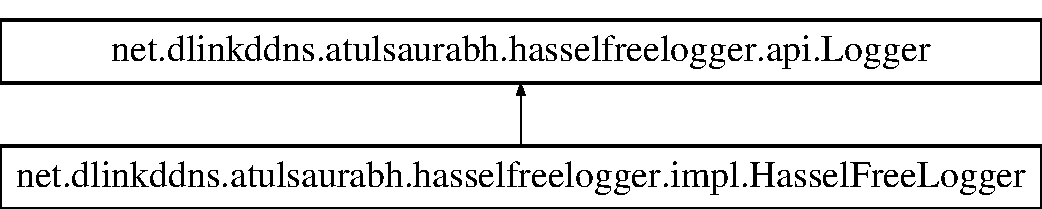
\includegraphics[height=2.000000cm]{d7/d4f/interfacenet_1_1dlinkddns_1_1atulsaurabh_1_1hasselfreelogger_1_1api_1_1_logger}
\end{center}
\end{figure}
\subsection*{Public Member Functions}
\begin{DoxyCompactItemize}
\item 
void \mbox{\hyperlink{interfacenet_1_1dlinkddns_1_1atulsaurabh_1_1hasselfreelogger_1_1api_1_1_logger_ae8fc6e4aeac87030546af120682aa178}{log\+Fatal}} (String message)
\item 
void \mbox{\hyperlink{interfacenet_1_1dlinkddns_1_1atulsaurabh_1_1hasselfreelogger_1_1api_1_1_logger_a05f87f45fe4302254060a2dac3429207}{log\+Fatal}} (Class error\+Class, String message)
\item 
void \mbox{\hyperlink{interfacenet_1_1dlinkddns_1_1atulsaurabh_1_1hasselfreelogger_1_1api_1_1_logger_a9ac7490ed937913b6dd97ee8898119bb}{log\+Fatal}} (Class error\+Class, String message, Throwable throwable)
\item 
void \mbox{\hyperlink{interfacenet_1_1dlinkddns_1_1atulsaurabh_1_1hasselfreelogger_1_1api_1_1_logger_a800f4847161a507a83b0d6731a01c210}{log\+All}} (String message)
\item 
void \mbox{\hyperlink{interfacenet_1_1dlinkddns_1_1atulsaurabh_1_1hasselfreelogger_1_1api_1_1_logger_ab5766fc9b8c0c78851d5ea90ade467b7}{log\+All}} (Class error\+Class, String message)
\item 
void \mbox{\hyperlink{interfacenet_1_1dlinkddns_1_1atulsaurabh_1_1hasselfreelogger_1_1api_1_1_logger_ad4c20aef678e51ab4822f5c301103f00}{log\+All}} (Class error\+Class, String message, Throwable throwable)
\item 
void \mbox{\hyperlink{interfacenet_1_1dlinkddns_1_1atulsaurabh_1_1hasselfreelogger_1_1api_1_1_logger_a2f15f4d94258528efb2938323deb8135}{set\+Rolling\+On}} (boolean rollingon)
\item 
boolean \mbox{\hyperlink{interfacenet_1_1dlinkddns_1_1atulsaurabh_1_1hasselfreelogger_1_1api_1_1_logger_a3815e1c6e6688af733cd8d098891c6da}{is\+Rolling\+On}} ()
\item 
void \mbox{\hyperlink{interfacenet_1_1dlinkddns_1_1atulsaurabh_1_1hasselfreelogger_1_1api_1_1_logger_a80727ab10655fa0ca0c5249ec3ed45b8}{set\+Date\+Pattern}} (String pattern)
\item 
String \mbox{\hyperlink{interfacenet_1_1dlinkddns_1_1atulsaurabh_1_1hasselfreelogger_1_1api_1_1_logger_ae0413346b180ceebfe7b522ed414a8ae}{get\+Date\+Pattern}} ()
\item 
void \mbox{\hyperlink{interfacenet_1_1dlinkddns_1_1atulsaurabh_1_1hasselfreelogger_1_1api_1_1_logger_a5a1b9dac86c15782309e01d5327e4299}{set\+Conversion\+Pattern}} (String pattern)
\item 
String \mbox{\hyperlink{interfacenet_1_1dlinkddns_1_1atulsaurabh_1_1hasselfreelogger_1_1api_1_1_logger_af32cfe36f98ae7223ab0ec37fc6c67f5}{get\+Conversion\+Pattern}} ()
\item 
void \mbox{\hyperlink{interfacenet_1_1dlinkddns_1_1atulsaurabh_1_1hasselfreelogger_1_1api_1_1_logger_a7a267e7aa9c678bdb6a3a7ca02a10efd}{log\+Warning}} (String message)
\item 
void \mbox{\hyperlink{interfacenet_1_1dlinkddns_1_1atulsaurabh_1_1hasselfreelogger_1_1api_1_1_logger_a2db4a8f0188cecd4ba6780b31136ded8}{log\+Warning}} (Class warning\+Class, String message)
\item 
void \mbox{\hyperlink{interfacenet_1_1dlinkddns_1_1atulsaurabh_1_1hasselfreelogger_1_1api_1_1_logger_af0535a8b640adb65e6830468b327d1da}{log\+Warning}} (Class warning\+Class, String message, Throwable throwable)
\item 
void \mbox{\hyperlink{interfacenet_1_1dlinkddns_1_1atulsaurabh_1_1hasselfreelogger_1_1api_1_1_logger_a90d0ff9fde52620be6884f4dee4ba00f}{log\+Info}} (String message)
\item 
void \mbox{\hyperlink{interfacenet_1_1dlinkddns_1_1atulsaurabh_1_1hasselfreelogger_1_1api_1_1_logger_ac0c7463bc249c77cd33e02b99a77a8d8}{log\+Info}} (Class info\+Class, String message)
\item 
void \mbox{\hyperlink{interfacenet_1_1dlinkddns_1_1atulsaurabh_1_1hasselfreelogger_1_1api_1_1_logger_a07cf4314c71f95135245d10dffc14d2f}{log\+Info}} (Class info\+Class, String message, Throwable throwable)
\item 
void \mbox{\hyperlink{interfacenet_1_1dlinkddns_1_1atulsaurabh_1_1hasselfreelogger_1_1api_1_1_logger_aabcbfa63158adde4db9d5735ef47663c}{log\+Debug}} (String message)
\item 
void \mbox{\hyperlink{interfacenet_1_1dlinkddns_1_1atulsaurabh_1_1hasselfreelogger_1_1api_1_1_logger_a029beee59dc44362c279f0a067dd0703}{log\+Debug}} (Class debug\+Class, String message)
\item 
void \mbox{\hyperlink{interfacenet_1_1dlinkddns_1_1atulsaurabh_1_1hasselfreelogger_1_1api_1_1_logger_aff388bb623493721b9aac70ef39492ec}{log\+Debug}} (Class debug\+Class, String message, Throwable throwable)
\item 
void \mbox{\hyperlink{interfacenet_1_1dlinkddns_1_1atulsaurabh_1_1hasselfreelogger_1_1api_1_1_logger_ae6a2cef332dfb10951c4cbfd822bbb63}{log\+Error}} (String message)
\item 
void \mbox{\hyperlink{interfacenet_1_1dlinkddns_1_1atulsaurabh_1_1hasselfreelogger_1_1api_1_1_logger_adf72322be1f6a5eaf0cf1b491b430b06}{log\+Error}} (Class error\+Class, String message)
\item 
void \mbox{\hyperlink{interfacenet_1_1dlinkddns_1_1atulsaurabh_1_1hasselfreelogger_1_1api_1_1_logger_a387cbc7fc16609202f2c63e88233ba49}{log\+Error}} (Class error\+Class, String message, Throwable throwable)
\item 
void \mbox{\hyperlink{interfacenet_1_1dlinkddns_1_1atulsaurabh_1_1hasselfreelogger_1_1api_1_1_logger_abe93800e399a9836cb92e6cb902a4ad8}{set\+Configuration}} (Properties properties)
\end{DoxyCompactItemize}


\subsection{Detailed Description}
\begin{DoxyAuthor}{Author}
Atul Saurabh 
\end{DoxyAuthor}
\begin{DoxyVersion}{Version}
1.\+0 
\end{DoxyVersion}


Definition at line 15 of file Logger.\+java.



\subsection{Member Function Documentation}
\mbox{\Hypertarget{interfacenet_1_1dlinkddns_1_1atulsaurabh_1_1hasselfreelogger_1_1api_1_1_logger_af32cfe36f98ae7223ab0ec37fc6c67f5}\label{interfacenet_1_1dlinkddns_1_1atulsaurabh_1_1hasselfreelogger_1_1api_1_1_logger_af32cfe36f98ae7223ab0ec37fc6c67f5}} 
\index{net\+::dlinkddns\+::atulsaurabh\+::hasselfreelogger\+::api\+::\+Logger@{net\+::dlinkddns\+::atulsaurabh\+::hasselfreelogger\+::api\+::\+Logger}!get\+Conversion\+Pattern@{get\+Conversion\+Pattern}}
\index{get\+Conversion\+Pattern@{get\+Conversion\+Pattern}!net\+::dlinkddns\+::atulsaurabh\+::hasselfreelogger\+::api\+::\+Logger@{net\+::dlinkddns\+::atulsaurabh\+::hasselfreelogger\+::api\+::\+Logger}}
\subsubsection{\texorpdfstring{get\+Conversion\+Pattern()}{getConversionPattern()}}
{\footnotesize\ttfamily String net.\+dlinkddns.\+atulsaurabh.\+hasselfreelogger.\+api.\+Logger.\+get\+Conversion\+Pattern (\begin{DoxyParamCaption}{ }\end{DoxyParamCaption})}

\begin{DoxyReturn}{Returns}
Format for printing message into log file 
\end{DoxyReturn}


Implemented in \mbox{\hyperlink{classnet_1_1dlinkddns_1_1atulsaurabh_1_1hasselfreelogger_1_1impl_1_1_hassel_free_logger_a8309e8b9abe877ce11e6b04faf48e8c1}{net.\+dlinkddns.\+atulsaurabh.\+hasselfreelogger.\+impl.\+Hassel\+Free\+Logger}}.

\mbox{\Hypertarget{interfacenet_1_1dlinkddns_1_1atulsaurabh_1_1hasselfreelogger_1_1api_1_1_logger_ae0413346b180ceebfe7b522ed414a8ae}\label{interfacenet_1_1dlinkddns_1_1atulsaurabh_1_1hasselfreelogger_1_1api_1_1_logger_ae0413346b180ceebfe7b522ed414a8ae}} 
\index{net\+::dlinkddns\+::atulsaurabh\+::hasselfreelogger\+::api\+::\+Logger@{net\+::dlinkddns\+::atulsaurabh\+::hasselfreelogger\+::api\+::\+Logger}!get\+Date\+Pattern@{get\+Date\+Pattern}}
\index{get\+Date\+Pattern@{get\+Date\+Pattern}!net\+::dlinkddns\+::atulsaurabh\+::hasselfreelogger\+::api\+::\+Logger@{net\+::dlinkddns\+::atulsaurabh\+::hasselfreelogger\+::api\+::\+Logger}}
\subsubsection{\texorpdfstring{get\+Date\+Pattern()}{getDatePattern()}}
{\footnotesize\ttfamily String net.\+dlinkddns.\+atulsaurabh.\+hasselfreelogger.\+api.\+Logger.\+get\+Date\+Pattern (\begin{DoxyParamCaption}{ }\end{DoxyParamCaption})}

\begin{DoxyReturn}{Returns}
date format used in log file 
\end{DoxyReturn}


Implemented in \mbox{\hyperlink{classnet_1_1dlinkddns_1_1atulsaurabh_1_1hasselfreelogger_1_1impl_1_1_hassel_free_logger_a9b56e6059627b493e8f5ebff888795a0}{net.\+dlinkddns.\+atulsaurabh.\+hasselfreelogger.\+impl.\+Hassel\+Free\+Logger}}.

\mbox{\Hypertarget{interfacenet_1_1dlinkddns_1_1atulsaurabh_1_1hasselfreelogger_1_1api_1_1_logger_a3815e1c6e6688af733cd8d098891c6da}\label{interfacenet_1_1dlinkddns_1_1atulsaurabh_1_1hasselfreelogger_1_1api_1_1_logger_a3815e1c6e6688af733cd8d098891c6da}} 
\index{net\+::dlinkddns\+::atulsaurabh\+::hasselfreelogger\+::api\+::\+Logger@{net\+::dlinkddns\+::atulsaurabh\+::hasselfreelogger\+::api\+::\+Logger}!is\+Rolling\+On@{is\+Rolling\+On}}
\index{is\+Rolling\+On@{is\+Rolling\+On}!net\+::dlinkddns\+::atulsaurabh\+::hasselfreelogger\+::api\+::\+Logger@{net\+::dlinkddns\+::atulsaurabh\+::hasselfreelogger\+::api\+::\+Logger}}
\subsubsection{\texorpdfstring{is\+Rolling\+On()}{isRollingOn()}}
{\footnotesize\ttfamily boolean net.\+dlinkddns.\+atulsaurabh.\+hasselfreelogger.\+api.\+Logger.\+is\+Rolling\+On (\begin{DoxyParamCaption}{ }\end{DoxyParamCaption})}

\begin{DoxyReturn}{Returns}
the state of rolling 
\end{DoxyReturn}


Implemented in \mbox{\hyperlink{classnet_1_1dlinkddns_1_1atulsaurabh_1_1hasselfreelogger_1_1impl_1_1_hassel_free_logger_a1264dcefa68828985aa843e545ff41b6}{net.\+dlinkddns.\+atulsaurabh.\+hasselfreelogger.\+impl.\+Hassel\+Free\+Logger}}.

\mbox{\Hypertarget{interfacenet_1_1dlinkddns_1_1atulsaurabh_1_1hasselfreelogger_1_1api_1_1_logger_a800f4847161a507a83b0d6731a01c210}\label{interfacenet_1_1dlinkddns_1_1atulsaurabh_1_1hasselfreelogger_1_1api_1_1_logger_a800f4847161a507a83b0d6731a01c210}} 
\index{net\+::dlinkddns\+::atulsaurabh\+::hasselfreelogger\+::api\+::\+Logger@{net\+::dlinkddns\+::atulsaurabh\+::hasselfreelogger\+::api\+::\+Logger}!log\+All@{log\+All}}
\index{log\+All@{log\+All}!net\+::dlinkddns\+::atulsaurabh\+::hasselfreelogger\+::api\+::\+Logger@{net\+::dlinkddns\+::atulsaurabh\+::hasselfreelogger\+::api\+::\+Logger}}
\subsubsection{\texorpdfstring{log\+All()}{logAll()}\hspace{0.1cm}{\footnotesize\ttfamily [1/3]}}
{\footnotesize\ttfamily void net.\+dlinkddns.\+atulsaurabh.\+hasselfreelogger.\+api.\+Logger.\+log\+All (\begin{DoxyParamCaption}\item[{String}]{message }\end{DoxyParamCaption})}


\begin{DoxyParams}{Parameters}
{\em message} & Any message to be logged in \\
\hline
\end{DoxyParams}


Implemented in \mbox{\hyperlink{classnet_1_1dlinkddns_1_1atulsaurabh_1_1hasselfreelogger_1_1impl_1_1_hassel_free_logger_af433939b275c708e5334f56a6444e2af}{net.\+dlinkddns.\+atulsaurabh.\+hasselfreelogger.\+impl.\+Hassel\+Free\+Logger}}.

\mbox{\Hypertarget{interfacenet_1_1dlinkddns_1_1atulsaurabh_1_1hasselfreelogger_1_1api_1_1_logger_ab5766fc9b8c0c78851d5ea90ade467b7}\label{interfacenet_1_1dlinkddns_1_1atulsaurabh_1_1hasselfreelogger_1_1api_1_1_logger_ab5766fc9b8c0c78851d5ea90ade467b7}} 
\index{net\+::dlinkddns\+::atulsaurabh\+::hasselfreelogger\+::api\+::\+Logger@{net\+::dlinkddns\+::atulsaurabh\+::hasselfreelogger\+::api\+::\+Logger}!log\+All@{log\+All}}
\index{log\+All@{log\+All}!net\+::dlinkddns\+::atulsaurabh\+::hasselfreelogger\+::api\+::\+Logger@{net\+::dlinkddns\+::atulsaurabh\+::hasselfreelogger\+::api\+::\+Logger}}
\subsubsection{\texorpdfstring{log\+All()}{logAll()}\hspace{0.1cm}{\footnotesize\ttfamily [2/3]}}
{\footnotesize\ttfamily void net.\+dlinkddns.\+atulsaurabh.\+hasselfreelogger.\+api.\+Logger.\+log\+All (\begin{DoxyParamCaption}\item[{Class}]{error\+Class,  }\item[{String}]{message }\end{DoxyParamCaption})}


\begin{DoxyParams}{Parameters}
{\em error\+Class} & Any error or warning or info etc generating class \\
\hline
{\em message} & Any message to be logged in \\
\hline
\end{DoxyParams}


Implemented in \mbox{\hyperlink{classnet_1_1dlinkddns_1_1atulsaurabh_1_1hasselfreelogger_1_1impl_1_1_hassel_free_logger_ade5a00300f3406a3a64ca003b1799dbd}{net.\+dlinkddns.\+atulsaurabh.\+hasselfreelogger.\+impl.\+Hassel\+Free\+Logger}}.

\mbox{\Hypertarget{interfacenet_1_1dlinkddns_1_1atulsaurabh_1_1hasselfreelogger_1_1api_1_1_logger_ad4c20aef678e51ab4822f5c301103f00}\label{interfacenet_1_1dlinkddns_1_1atulsaurabh_1_1hasselfreelogger_1_1api_1_1_logger_ad4c20aef678e51ab4822f5c301103f00}} 
\index{net\+::dlinkddns\+::atulsaurabh\+::hasselfreelogger\+::api\+::\+Logger@{net\+::dlinkddns\+::atulsaurabh\+::hasselfreelogger\+::api\+::\+Logger}!log\+All@{log\+All}}
\index{log\+All@{log\+All}!net\+::dlinkddns\+::atulsaurabh\+::hasselfreelogger\+::api\+::\+Logger@{net\+::dlinkddns\+::atulsaurabh\+::hasselfreelogger\+::api\+::\+Logger}}
\subsubsection{\texorpdfstring{log\+All()}{logAll()}\hspace{0.1cm}{\footnotesize\ttfamily [3/3]}}
{\footnotesize\ttfamily void net.\+dlinkddns.\+atulsaurabh.\+hasselfreelogger.\+api.\+Logger.\+log\+All (\begin{DoxyParamCaption}\item[{Class}]{error\+Class,  }\item[{String}]{message,  }\item[{Throwable}]{throwable }\end{DoxyParamCaption})}


\begin{DoxyParams}{Parameters}
{\em error\+Class} & Any error or warning or info etc generating class \\
\hline
{\em message} & Any message to be logged in \\
\hline
{\em throwable} & Any object representing warning,error,fatal etc. \\
\hline
\end{DoxyParams}


Implemented in \mbox{\hyperlink{classnet_1_1dlinkddns_1_1atulsaurabh_1_1hasselfreelogger_1_1impl_1_1_hassel_free_logger_a6b63592b0c825713f2bc861b6d487df8}{net.\+dlinkddns.\+atulsaurabh.\+hasselfreelogger.\+impl.\+Hassel\+Free\+Logger}}.

\mbox{\Hypertarget{interfacenet_1_1dlinkddns_1_1atulsaurabh_1_1hasselfreelogger_1_1api_1_1_logger_aabcbfa63158adde4db9d5735ef47663c}\label{interfacenet_1_1dlinkddns_1_1atulsaurabh_1_1hasselfreelogger_1_1api_1_1_logger_aabcbfa63158adde4db9d5735ef47663c}} 
\index{net\+::dlinkddns\+::atulsaurabh\+::hasselfreelogger\+::api\+::\+Logger@{net\+::dlinkddns\+::atulsaurabh\+::hasselfreelogger\+::api\+::\+Logger}!log\+Debug@{log\+Debug}}
\index{log\+Debug@{log\+Debug}!net\+::dlinkddns\+::atulsaurabh\+::hasselfreelogger\+::api\+::\+Logger@{net\+::dlinkddns\+::atulsaurabh\+::hasselfreelogger\+::api\+::\+Logger}}
\subsubsection{\texorpdfstring{log\+Debug()}{logDebug()}\hspace{0.1cm}{\footnotesize\ttfamily [1/3]}}
{\footnotesize\ttfamily void net.\+dlinkddns.\+atulsaurabh.\+hasselfreelogger.\+api.\+Logger.\+log\+Debug (\begin{DoxyParamCaption}\item[{String}]{message }\end{DoxyParamCaption})}



Implemented in \mbox{\hyperlink{classnet_1_1dlinkddns_1_1atulsaurabh_1_1hasselfreelogger_1_1impl_1_1_hassel_free_logger_a7aafa489bd14255cbdb43c1f2494d433}{net.\+dlinkddns.\+atulsaurabh.\+hasselfreelogger.\+impl.\+Hassel\+Free\+Logger}}.

\mbox{\Hypertarget{interfacenet_1_1dlinkddns_1_1atulsaurabh_1_1hasselfreelogger_1_1api_1_1_logger_a029beee59dc44362c279f0a067dd0703}\label{interfacenet_1_1dlinkddns_1_1atulsaurabh_1_1hasselfreelogger_1_1api_1_1_logger_a029beee59dc44362c279f0a067dd0703}} 
\index{net\+::dlinkddns\+::atulsaurabh\+::hasselfreelogger\+::api\+::\+Logger@{net\+::dlinkddns\+::atulsaurabh\+::hasselfreelogger\+::api\+::\+Logger}!log\+Debug@{log\+Debug}}
\index{log\+Debug@{log\+Debug}!net\+::dlinkddns\+::atulsaurabh\+::hasselfreelogger\+::api\+::\+Logger@{net\+::dlinkddns\+::atulsaurabh\+::hasselfreelogger\+::api\+::\+Logger}}
\subsubsection{\texorpdfstring{log\+Debug()}{logDebug()}\hspace{0.1cm}{\footnotesize\ttfamily [2/3]}}
{\footnotesize\ttfamily void net.\+dlinkddns.\+atulsaurabh.\+hasselfreelogger.\+api.\+Logger.\+log\+Debug (\begin{DoxyParamCaption}\item[{Class}]{debug\+Class,  }\item[{String}]{message }\end{DoxyParamCaption})}



Implemented in \mbox{\hyperlink{classnet_1_1dlinkddns_1_1atulsaurabh_1_1hasselfreelogger_1_1impl_1_1_hassel_free_logger_a7c65f65791b715d7c72a2227a8a00bdc}{net.\+dlinkddns.\+atulsaurabh.\+hasselfreelogger.\+impl.\+Hassel\+Free\+Logger}}.

\mbox{\Hypertarget{interfacenet_1_1dlinkddns_1_1atulsaurabh_1_1hasselfreelogger_1_1api_1_1_logger_aff388bb623493721b9aac70ef39492ec}\label{interfacenet_1_1dlinkddns_1_1atulsaurabh_1_1hasselfreelogger_1_1api_1_1_logger_aff388bb623493721b9aac70ef39492ec}} 
\index{net\+::dlinkddns\+::atulsaurabh\+::hasselfreelogger\+::api\+::\+Logger@{net\+::dlinkddns\+::atulsaurabh\+::hasselfreelogger\+::api\+::\+Logger}!log\+Debug@{log\+Debug}}
\index{log\+Debug@{log\+Debug}!net\+::dlinkddns\+::atulsaurabh\+::hasselfreelogger\+::api\+::\+Logger@{net\+::dlinkddns\+::atulsaurabh\+::hasselfreelogger\+::api\+::\+Logger}}
\subsubsection{\texorpdfstring{log\+Debug()}{logDebug()}\hspace{0.1cm}{\footnotesize\ttfamily [3/3]}}
{\footnotesize\ttfamily void net.\+dlinkddns.\+atulsaurabh.\+hasselfreelogger.\+api.\+Logger.\+log\+Debug (\begin{DoxyParamCaption}\item[{Class}]{debug\+Class,  }\item[{String}]{message,  }\item[{Throwable}]{throwable }\end{DoxyParamCaption})}



Implemented in \mbox{\hyperlink{classnet_1_1dlinkddns_1_1atulsaurabh_1_1hasselfreelogger_1_1impl_1_1_hassel_free_logger_a0995d59f7b5262af4be98f4e7ba21cd0}{net.\+dlinkddns.\+atulsaurabh.\+hasselfreelogger.\+impl.\+Hassel\+Free\+Logger}}.

\mbox{\Hypertarget{interfacenet_1_1dlinkddns_1_1atulsaurabh_1_1hasselfreelogger_1_1api_1_1_logger_ae6a2cef332dfb10951c4cbfd822bbb63}\label{interfacenet_1_1dlinkddns_1_1atulsaurabh_1_1hasselfreelogger_1_1api_1_1_logger_ae6a2cef332dfb10951c4cbfd822bbb63}} 
\index{net\+::dlinkddns\+::atulsaurabh\+::hasselfreelogger\+::api\+::\+Logger@{net\+::dlinkddns\+::atulsaurabh\+::hasselfreelogger\+::api\+::\+Logger}!log\+Error@{log\+Error}}
\index{log\+Error@{log\+Error}!net\+::dlinkddns\+::atulsaurabh\+::hasselfreelogger\+::api\+::\+Logger@{net\+::dlinkddns\+::atulsaurabh\+::hasselfreelogger\+::api\+::\+Logger}}
\subsubsection{\texorpdfstring{log\+Error()}{logError()}\hspace{0.1cm}{\footnotesize\ttfamily [1/3]}}
{\footnotesize\ttfamily void net.\+dlinkddns.\+atulsaurabh.\+hasselfreelogger.\+api.\+Logger.\+log\+Error (\begin{DoxyParamCaption}\item[{String}]{message }\end{DoxyParamCaption})}



Implemented in \mbox{\hyperlink{classnet_1_1dlinkddns_1_1atulsaurabh_1_1hasselfreelogger_1_1impl_1_1_hassel_free_logger_a94641af9c6c39ea601d5c41bf68a4b1f}{net.\+dlinkddns.\+atulsaurabh.\+hasselfreelogger.\+impl.\+Hassel\+Free\+Logger}}.

\mbox{\Hypertarget{interfacenet_1_1dlinkddns_1_1atulsaurabh_1_1hasselfreelogger_1_1api_1_1_logger_adf72322be1f6a5eaf0cf1b491b430b06}\label{interfacenet_1_1dlinkddns_1_1atulsaurabh_1_1hasselfreelogger_1_1api_1_1_logger_adf72322be1f6a5eaf0cf1b491b430b06}} 
\index{net\+::dlinkddns\+::atulsaurabh\+::hasselfreelogger\+::api\+::\+Logger@{net\+::dlinkddns\+::atulsaurabh\+::hasselfreelogger\+::api\+::\+Logger}!log\+Error@{log\+Error}}
\index{log\+Error@{log\+Error}!net\+::dlinkddns\+::atulsaurabh\+::hasselfreelogger\+::api\+::\+Logger@{net\+::dlinkddns\+::atulsaurabh\+::hasselfreelogger\+::api\+::\+Logger}}
\subsubsection{\texorpdfstring{log\+Error()}{logError()}\hspace{0.1cm}{\footnotesize\ttfamily [2/3]}}
{\footnotesize\ttfamily void net.\+dlinkddns.\+atulsaurabh.\+hasselfreelogger.\+api.\+Logger.\+log\+Error (\begin{DoxyParamCaption}\item[{Class}]{error\+Class,  }\item[{String}]{message }\end{DoxyParamCaption})}



Implemented in \mbox{\hyperlink{classnet_1_1dlinkddns_1_1atulsaurabh_1_1hasselfreelogger_1_1impl_1_1_hassel_free_logger_a47870e52004c823f0ef365f5d41afd6b}{net.\+dlinkddns.\+atulsaurabh.\+hasselfreelogger.\+impl.\+Hassel\+Free\+Logger}}.

\mbox{\Hypertarget{interfacenet_1_1dlinkddns_1_1atulsaurabh_1_1hasselfreelogger_1_1api_1_1_logger_a387cbc7fc16609202f2c63e88233ba49}\label{interfacenet_1_1dlinkddns_1_1atulsaurabh_1_1hasselfreelogger_1_1api_1_1_logger_a387cbc7fc16609202f2c63e88233ba49}} 
\index{net\+::dlinkddns\+::atulsaurabh\+::hasselfreelogger\+::api\+::\+Logger@{net\+::dlinkddns\+::atulsaurabh\+::hasselfreelogger\+::api\+::\+Logger}!log\+Error@{log\+Error}}
\index{log\+Error@{log\+Error}!net\+::dlinkddns\+::atulsaurabh\+::hasselfreelogger\+::api\+::\+Logger@{net\+::dlinkddns\+::atulsaurabh\+::hasselfreelogger\+::api\+::\+Logger}}
\subsubsection{\texorpdfstring{log\+Error()}{logError()}\hspace{0.1cm}{\footnotesize\ttfamily [3/3]}}
{\footnotesize\ttfamily void net.\+dlinkddns.\+atulsaurabh.\+hasselfreelogger.\+api.\+Logger.\+log\+Error (\begin{DoxyParamCaption}\item[{Class}]{error\+Class,  }\item[{String}]{message,  }\item[{Throwable}]{throwable }\end{DoxyParamCaption})}



Implemented in \mbox{\hyperlink{classnet_1_1dlinkddns_1_1atulsaurabh_1_1hasselfreelogger_1_1impl_1_1_hassel_free_logger_acf886c01c94bba98b551f98e2ad8ce4f}{net.\+dlinkddns.\+atulsaurabh.\+hasselfreelogger.\+impl.\+Hassel\+Free\+Logger}}.

\mbox{\Hypertarget{interfacenet_1_1dlinkddns_1_1atulsaurabh_1_1hasselfreelogger_1_1api_1_1_logger_ae8fc6e4aeac87030546af120682aa178}\label{interfacenet_1_1dlinkddns_1_1atulsaurabh_1_1hasselfreelogger_1_1api_1_1_logger_ae8fc6e4aeac87030546af120682aa178}} 
\index{net\+::dlinkddns\+::atulsaurabh\+::hasselfreelogger\+::api\+::\+Logger@{net\+::dlinkddns\+::atulsaurabh\+::hasselfreelogger\+::api\+::\+Logger}!log\+Fatal@{log\+Fatal}}
\index{log\+Fatal@{log\+Fatal}!net\+::dlinkddns\+::atulsaurabh\+::hasselfreelogger\+::api\+::\+Logger@{net\+::dlinkddns\+::atulsaurabh\+::hasselfreelogger\+::api\+::\+Logger}}
\subsubsection{\texorpdfstring{log\+Fatal()}{logFatal()}\hspace{0.1cm}{\footnotesize\ttfamily [1/3]}}
{\footnotesize\ttfamily void net.\+dlinkddns.\+atulsaurabh.\+hasselfreelogger.\+api.\+Logger.\+log\+Fatal (\begin{DoxyParamCaption}\item[{String}]{message }\end{DoxyParamCaption})}


\begin{DoxyParams}{Parameters}
{\em message} & Fatal message to be logged \\
\hline
\end{DoxyParams}


Implemented in \mbox{\hyperlink{classnet_1_1dlinkddns_1_1atulsaurabh_1_1hasselfreelogger_1_1impl_1_1_hassel_free_logger_a478d877ebdbb5cb2796ad23d0dafe369}{net.\+dlinkddns.\+atulsaurabh.\+hasselfreelogger.\+impl.\+Hassel\+Free\+Logger}}.

\mbox{\Hypertarget{interfacenet_1_1dlinkddns_1_1atulsaurabh_1_1hasselfreelogger_1_1api_1_1_logger_a05f87f45fe4302254060a2dac3429207}\label{interfacenet_1_1dlinkddns_1_1atulsaurabh_1_1hasselfreelogger_1_1api_1_1_logger_a05f87f45fe4302254060a2dac3429207}} 
\index{net\+::dlinkddns\+::atulsaurabh\+::hasselfreelogger\+::api\+::\+Logger@{net\+::dlinkddns\+::atulsaurabh\+::hasselfreelogger\+::api\+::\+Logger}!log\+Fatal@{log\+Fatal}}
\index{log\+Fatal@{log\+Fatal}!net\+::dlinkddns\+::atulsaurabh\+::hasselfreelogger\+::api\+::\+Logger@{net\+::dlinkddns\+::atulsaurabh\+::hasselfreelogger\+::api\+::\+Logger}}
\subsubsection{\texorpdfstring{log\+Fatal()}{logFatal()}\hspace{0.1cm}{\footnotesize\ttfamily [2/3]}}
{\footnotesize\ttfamily void net.\+dlinkddns.\+atulsaurabh.\+hasselfreelogger.\+api.\+Logger.\+log\+Fatal (\begin{DoxyParamCaption}\item[{Class}]{error\+Class,  }\item[{String}]{message }\end{DoxyParamCaption})}


\begin{DoxyParams}{Parameters}
{\em error\+Class} & Class where exception is caught \\
\hline
{\em message} & Fatal message to be logged \\
\hline
\end{DoxyParams}


Implemented in \mbox{\hyperlink{classnet_1_1dlinkddns_1_1atulsaurabh_1_1hasselfreelogger_1_1impl_1_1_hassel_free_logger_a40d4e893854bc742145dbf2fe5d2aa43}{net.\+dlinkddns.\+atulsaurabh.\+hasselfreelogger.\+impl.\+Hassel\+Free\+Logger}}.

\mbox{\Hypertarget{interfacenet_1_1dlinkddns_1_1atulsaurabh_1_1hasselfreelogger_1_1api_1_1_logger_a9ac7490ed937913b6dd97ee8898119bb}\label{interfacenet_1_1dlinkddns_1_1atulsaurabh_1_1hasselfreelogger_1_1api_1_1_logger_a9ac7490ed937913b6dd97ee8898119bb}} 
\index{net\+::dlinkddns\+::atulsaurabh\+::hasselfreelogger\+::api\+::\+Logger@{net\+::dlinkddns\+::atulsaurabh\+::hasselfreelogger\+::api\+::\+Logger}!log\+Fatal@{log\+Fatal}}
\index{log\+Fatal@{log\+Fatal}!net\+::dlinkddns\+::atulsaurabh\+::hasselfreelogger\+::api\+::\+Logger@{net\+::dlinkddns\+::atulsaurabh\+::hasselfreelogger\+::api\+::\+Logger}}
\subsubsection{\texorpdfstring{log\+Fatal()}{logFatal()}\hspace{0.1cm}{\footnotesize\ttfamily [3/3]}}
{\footnotesize\ttfamily void net.\+dlinkddns.\+atulsaurabh.\+hasselfreelogger.\+api.\+Logger.\+log\+Fatal (\begin{DoxyParamCaption}\item[{Class}]{error\+Class,  }\item[{String}]{message,  }\item[{Throwable}]{throwable }\end{DoxyParamCaption})}


\begin{DoxyParams}{Parameters}
{\em error\+Class} & Class where exception is caught \\
\hline
{\em message} & Fatal message to be logged \\
\hline
{\em throwable} & The instance of exception generated from stack trace \\
\hline
\end{DoxyParams}


Implemented in \mbox{\hyperlink{classnet_1_1dlinkddns_1_1atulsaurabh_1_1hasselfreelogger_1_1impl_1_1_hassel_free_logger_a546bc74e8eec8333893e294a98bbe939}{net.\+dlinkddns.\+atulsaurabh.\+hasselfreelogger.\+impl.\+Hassel\+Free\+Logger}}.

\mbox{\Hypertarget{interfacenet_1_1dlinkddns_1_1atulsaurabh_1_1hasselfreelogger_1_1api_1_1_logger_a90d0ff9fde52620be6884f4dee4ba00f}\label{interfacenet_1_1dlinkddns_1_1atulsaurabh_1_1hasselfreelogger_1_1api_1_1_logger_a90d0ff9fde52620be6884f4dee4ba00f}} 
\index{net\+::dlinkddns\+::atulsaurabh\+::hasselfreelogger\+::api\+::\+Logger@{net\+::dlinkddns\+::atulsaurabh\+::hasselfreelogger\+::api\+::\+Logger}!log\+Info@{log\+Info}}
\index{log\+Info@{log\+Info}!net\+::dlinkddns\+::atulsaurabh\+::hasselfreelogger\+::api\+::\+Logger@{net\+::dlinkddns\+::atulsaurabh\+::hasselfreelogger\+::api\+::\+Logger}}
\subsubsection{\texorpdfstring{log\+Info()}{logInfo()}\hspace{0.1cm}{\footnotesize\ttfamily [1/3]}}
{\footnotesize\ttfamily void net.\+dlinkddns.\+atulsaurabh.\+hasselfreelogger.\+api.\+Logger.\+log\+Info (\begin{DoxyParamCaption}\item[{String}]{message }\end{DoxyParamCaption})}



Implemented in \mbox{\hyperlink{classnet_1_1dlinkddns_1_1atulsaurabh_1_1hasselfreelogger_1_1impl_1_1_hassel_free_logger_abca8e8a8a8c85d582092b35fc395d726}{net.\+dlinkddns.\+atulsaurabh.\+hasselfreelogger.\+impl.\+Hassel\+Free\+Logger}}.

\mbox{\Hypertarget{interfacenet_1_1dlinkddns_1_1atulsaurabh_1_1hasselfreelogger_1_1api_1_1_logger_ac0c7463bc249c77cd33e02b99a77a8d8}\label{interfacenet_1_1dlinkddns_1_1atulsaurabh_1_1hasselfreelogger_1_1api_1_1_logger_ac0c7463bc249c77cd33e02b99a77a8d8}} 
\index{net\+::dlinkddns\+::atulsaurabh\+::hasselfreelogger\+::api\+::\+Logger@{net\+::dlinkddns\+::atulsaurabh\+::hasselfreelogger\+::api\+::\+Logger}!log\+Info@{log\+Info}}
\index{log\+Info@{log\+Info}!net\+::dlinkddns\+::atulsaurabh\+::hasselfreelogger\+::api\+::\+Logger@{net\+::dlinkddns\+::atulsaurabh\+::hasselfreelogger\+::api\+::\+Logger}}
\subsubsection{\texorpdfstring{log\+Info()}{logInfo()}\hspace{0.1cm}{\footnotesize\ttfamily [2/3]}}
{\footnotesize\ttfamily void net.\+dlinkddns.\+atulsaurabh.\+hasselfreelogger.\+api.\+Logger.\+log\+Info (\begin{DoxyParamCaption}\item[{Class}]{info\+Class,  }\item[{String}]{message }\end{DoxyParamCaption})}



Implemented in \mbox{\hyperlink{classnet_1_1dlinkddns_1_1atulsaurabh_1_1hasselfreelogger_1_1impl_1_1_hassel_free_logger_a011e8791e13b815927a16254e9cfa2a3}{net.\+dlinkddns.\+atulsaurabh.\+hasselfreelogger.\+impl.\+Hassel\+Free\+Logger}}.

\mbox{\Hypertarget{interfacenet_1_1dlinkddns_1_1atulsaurabh_1_1hasselfreelogger_1_1api_1_1_logger_a07cf4314c71f95135245d10dffc14d2f}\label{interfacenet_1_1dlinkddns_1_1atulsaurabh_1_1hasselfreelogger_1_1api_1_1_logger_a07cf4314c71f95135245d10dffc14d2f}} 
\index{net\+::dlinkddns\+::atulsaurabh\+::hasselfreelogger\+::api\+::\+Logger@{net\+::dlinkddns\+::atulsaurabh\+::hasselfreelogger\+::api\+::\+Logger}!log\+Info@{log\+Info}}
\index{log\+Info@{log\+Info}!net\+::dlinkddns\+::atulsaurabh\+::hasselfreelogger\+::api\+::\+Logger@{net\+::dlinkddns\+::atulsaurabh\+::hasselfreelogger\+::api\+::\+Logger}}
\subsubsection{\texorpdfstring{log\+Info()}{logInfo()}\hspace{0.1cm}{\footnotesize\ttfamily [3/3]}}
{\footnotesize\ttfamily void net.\+dlinkddns.\+atulsaurabh.\+hasselfreelogger.\+api.\+Logger.\+log\+Info (\begin{DoxyParamCaption}\item[{Class}]{info\+Class,  }\item[{String}]{message,  }\item[{Throwable}]{throwable }\end{DoxyParamCaption})}



Implemented in \mbox{\hyperlink{classnet_1_1dlinkddns_1_1atulsaurabh_1_1hasselfreelogger_1_1impl_1_1_hassel_free_logger_ac0596a92805b29d9402a9eb17c71891a}{net.\+dlinkddns.\+atulsaurabh.\+hasselfreelogger.\+impl.\+Hassel\+Free\+Logger}}.

\mbox{\Hypertarget{interfacenet_1_1dlinkddns_1_1atulsaurabh_1_1hasselfreelogger_1_1api_1_1_logger_a7a267e7aa9c678bdb6a3a7ca02a10efd}\label{interfacenet_1_1dlinkddns_1_1atulsaurabh_1_1hasselfreelogger_1_1api_1_1_logger_a7a267e7aa9c678bdb6a3a7ca02a10efd}} 
\index{net\+::dlinkddns\+::atulsaurabh\+::hasselfreelogger\+::api\+::\+Logger@{net\+::dlinkddns\+::atulsaurabh\+::hasselfreelogger\+::api\+::\+Logger}!log\+Warning@{log\+Warning}}
\index{log\+Warning@{log\+Warning}!net\+::dlinkddns\+::atulsaurabh\+::hasselfreelogger\+::api\+::\+Logger@{net\+::dlinkddns\+::atulsaurabh\+::hasselfreelogger\+::api\+::\+Logger}}
\subsubsection{\texorpdfstring{log\+Warning()}{logWarning()}\hspace{0.1cm}{\footnotesize\ttfamily [1/3]}}
{\footnotesize\ttfamily void net.\+dlinkddns.\+atulsaurabh.\+hasselfreelogger.\+api.\+Logger.\+log\+Warning (\begin{DoxyParamCaption}\item[{String}]{message }\end{DoxyParamCaption})}



Implemented in \mbox{\hyperlink{classnet_1_1dlinkddns_1_1atulsaurabh_1_1hasselfreelogger_1_1impl_1_1_hassel_free_logger_a9e847886284d6a0f7edef691e2d11efd}{net.\+dlinkddns.\+atulsaurabh.\+hasselfreelogger.\+impl.\+Hassel\+Free\+Logger}}.

\mbox{\Hypertarget{interfacenet_1_1dlinkddns_1_1atulsaurabh_1_1hasselfreelogger_1_1api_1_1_logger_a2db4a8f0188cecd4ba6780b31136ded8}\label{interfacenet_1_1dlinkddns_1_1atulsaurabh_1_1hasselfreelogger_1_1api_1_1_logger_a2db4a8f0188cecd4ba6780b31136ded8}} 
\index{net\+::dlinkddns\+::atulsaurabh\+::hasselfreelogger\+::api\+::\+Logger@{net\+::dlinkddns\+::atulsaurabh\+::hasselfreelogger\+::api\+::\+Logger}!log\+Warning@{log\+Warning}}
\index{log\+Warning@{log\+Warning}!net\+::dlinkddns\+::atulsaurabh\+::hasselfreelogger\+::api\+::\+Logger@{net\+::dlinkddns\+::atulsaurabh\+::hasselfreelogger\+::api\+::\+Logger}}
\subsubsection{\texorpdfstring{log\+Warning()}{logWarning()}\hspace{0.1cm}{\footnotesize\ttfamily [2/3]}}
{\footnotesize\ttfamily void net.\+dlinkddns.\+atulsaurabh.\+hasselfreelogger.\+api.\+Logger.\+log\+Warning (\begin{DoxyParamCaption}\item[{Class}]{warning\+Class,  }\item[{String}]{message }\end{DoxyParamCaption})}



Implemented in \mbox{\hyperlink{classnet_1_1dlinkddns_1_1atulsaurabh_1_1hasselfreelogger_1_1impl_1_1_hassel_free_logger_ad5f8400bc0ea2500509a4154cfa48bf5}{net.\+dlinkddns.\+atulsaurabh.\+hasselfreelogger.\+impl.\+Hassel\+Free\+Logger}}.

\mbox{\Hypertarget{interfacenet_1_1dlinkddns_1_1atulsaurabh_1_1hasselfreelogger_1_1api_1_1_logger_af0535a8b640adb65e6830468b327d1da}\label{interfacenet_1_1dlinkddns_1_1atulsaurabh_1_1hasselfreelogger_1_1api_1_1_logger_af0535a8b640adb65e6830468b327d1da}} 
\index{net\+::dlinkddns\+::atulsaurabh\+::hasselfreelogger\+::api\+::\+Logger@{net\+::dlinkddns\+::atulsaurabh\+::hasselfreelogger\+::api\+::\+Logger}!log\+Warning@{log\+Warning}}
\index{log\+Warning@{log\+Warning}!net\+::dlinkddns\+::atulsaurabh\+::hasselfreelogger\+::api\+::\+Logger@{net\+::dlinkddns\+::atulsaurabh\+::hasselfreelogger\+::api\+::\+Logger}}
\subsubsection{\texorpdfstring{log\+Warning()}{logWarning()}\hspace{0.1cm}{\footnotesize\ttfamily [3/3]}}
{\footnotesize\ttfamily void net.\+dlinkddns.\+atulsaurabh.\+hasselfreelogger.\+api.\+Logger.\+log\+Warning (\begin{DoxyParamCaption}\item[{Class}]{warning\+Class,  }\item[{String}]{message,  }\item[{Throwable}]{throwable }\end{DoxyParamCaption})}



Implemented in \mbox{\hyperlink{classnet_1_1dlinkddns_1_1atulsaurabh_1_1hasselfreelogger_1_1impl_1_1_hassel_free_logger_ac5e36ee2095f1f92c90885360a0fd1f1}{net.\+dlinkddns.\+atulsaurabh.\+hasselfreelogger.\+impl.\+Hassel\+Free\+Logger}}.

\mbox{\Hypertarget{interfacenet_1_1dlinkddns_1_1atulsaurabh_1_1hasselfreelogger_1_1api_1_1_logger_abe93800e399a9836cb92e6cb902a4ad8}\label{interfacenet_1_1dlinkddns_1_1atulsaurabh_1_1hasselfreelogger_1_1api_1_1_logger_abe93800e399a9836cb92e6cb902a4ad8}} 
\index{net\+::dlinkddns\+::atulsaurabh\+::hasselfreelogger\+::api\+::\+Logger@{net\+::dlinkddns\+::atulsaurabh\+::hasselfreelogger\+::api\+::\+Logger}!set\+Configuration@{set\+Configuration}}
\index{set\+Configuration@{set\+Configuration}!net\+::dlinkddns\+::atulsaurabh\+::hasselfreelogger\+::api\+::\+Logger@{net\+::dlinkddns\+::atulsaurabh\+::hasselfreelogger\+::api\+::\+Logger}}
\subsubsection{\texorpdfstring{set\+Configuration()}{setConfiguration()}}
{\footnotesize\ttfamily void net.\+dlinkddns.\+atulsaurabh.\+hasselfreelogger.\+api.\+Logger.\+set\+Configuration (\begin{DoxyParamCaption}\item[{Properties}]{properties }\end{DoxyParamCaption})}



Implemented in \mbox{\hyperlink{classnet_1_1dlinkddns_1_1atulsaurabh_1_1hasselfreelogger_1_1impl_1_1_hassel_free_logger_a9dbc7356642960679aaa76cc054ce456}{net.\+dlinkddns.\+atulsaurabh.\+hasselfreelogger.\+impl.\+Hassel\+Free\+Logger}}.

\mbox{\Hypertarget{interfacenet_1_1dlinkddns_1_1atulsaurabh_1_1hasselfreelogger_1_1api_1_1_logger_a5a1b9dac86c15782309e01d5327e4299}\label{interfacenet_1_1dlinkddns_1_1atulsaurabh_1_1hasselfreelogger_1_1api_1_1_logger_a5a1b9dac86c15782309e01d5327e4299}} 
\index{net\+::dlinkddns\+::atulsaurabh\+::hasselfreelogger\+::api\+::\+Logger@{net\+::dlinkddns\+::atulsaurabh\+::hasselfreelogger\+::api\+::\+Logger}!set\+Conversion\+Pattern@{set\+Conversion\+Pattern}}
\index{set\+Conversion\+Pattern@{set\+Conversion\+Pattern}!net\+::dlinkddns\+::atulsaurabh\+::hasselfreelogger\+::api\+::\+Logger@{net\+::dlinkddns\+::atulsaurabh\+::hasselfreelogger\+::api\+::\+Logger}}
\subsubsection{\texorpdfstring{set\+Conversion\+Pattern()}{setConversionPattern()}}
{\footnotesize\ttfamily void net.\+dlinkddns.\+atulsaurabh.\+hasselfreelogger.\+api.\+Logger.\+set\+Conversion\+Pattern (\begin{DoxyParamCaption}\item[{String}]{pattern }\end{DoxyParamCaption})}


\begin{DoxyParams}{Parameters}
{\em pattern} & Format for printing message into log file \\
\hline
\end{DoxyParams}


Implemented in \mbox{\hyperlink{classnet_1_1dlinkddns_1_1atulsaurabh_1_1hasselfreelogger_1_1impl_1_1_hassel_free_logger_a23a1e3b5c56528e197c7eb3832e7c69e}{net.\+dlinkddns.\+atulsaurabh.\+hasselfreelogger.\+impl.\+Hassel\+Free\+Logger}}.

\mbox{\Hypertarget{interfacenet_1_1dlinkddns_1_1atulsaurabh_1_1hasselfreelogger_1_1api_1_1_logger_a80727ab10655fa0ca0c5249ec3ed45b8}\label{interfacenet_1_1dlinkddns_1_1atulsaurabh_1_1hasselfreelogger_1_1api_1_1_logger_a80727ab10655fa0ca0c5249ec3ed45b8}} 
\index{net\+::dlinkddns\+::atulsaurabh\+::hasselfreelogger\+::api\+::\+Logger@{net\+::dlinkddns\+::atulsaurabh\+::hasselfreelogger\+::api\+::\+Logger}!set\+Date\+Pattern@{set\+Date\+Pattern}}
\index{set\+Date\+Pattern@{set\+Date\+Pattern}!net\+::dlinkddns\+::atulsaurabh\+::hasselfreelogger\+::api\+::\+Logger@{net\+::dlinkddns\+::atulsaurabh\+::hasselfreelogger\+::api\+::\+Logger}}
\subsubsection{\texorpdfstring{set\+Date\+Pattern()}{setDatePattern()}}
{\footnotesize\ttfamily void net.\+dlinkddns.\+atulsaurabh.\+hasselfreelogger.\+api.\+Logger.\+set\+Date\+Pattern (\begin{DoxyParamCaption}\item[{String}]{pattern }\end{DoxyParamCaption})}


\begin{DoxyParams}{Parameters}
{\em pattern} & The pattern for date used in log file \\
\hline
\end{DoxyParams}


Implemented in \mbox{\hyperlink{classnet_1_1dlinkddns_1_1atulsaurabh_1_1hasselfreelogger_1_1impl_1_1_hassel_free_logger_a72529568d69eea543b2238a466cedf8d}{net.\+dlinkddns.\+atulsaurabh.\+hasselfreelogger.\+impl.\+Hassel\+Free\+Logger}}.

\mbox{\Hypertarget{interfacenet_1_1dlinkddns_1_1atulsaurabh_1_1hasselfreelogger_1_1api_1_1_logger_a2f15f4d94258528efb2938323deb8135}\label{interfacenet_1_1dlinkddns_1_1atulsaurabh_1_1hasselfreelogger_1_1api_1_1_logger_a2f15f4d94258528efb2938323deb8135}} 
\index{net\+::dlinkddns\+::atulsaurabh\+::hasselfreelogger\+::api\+::\+Logger@{net\+::dlinkddns\+::atulsaurabh\+::hasselfreelogger\+::api\+::\+Logger}!set\+Rolling\+On@{set\+Rolling\+On}}
\index{set\+Rolling\+On@{set\+Rolling\+On}!net\+::dlinkddns\+::atulsaurabh\+::hasselfreelogger\+::api\+::\+Logger@{net\+::dlinkddns\+::atulsaurabh\+::hasselfreelogger\+::api\+::\+Logger}}
\subsubsection{\texorpdfstring{set\+Rolling\+On()}{setRollingOn()}}
{\footnotesize\ttfamily void net.\+dlinkddns.\+atulsaurabh.\+hasselfreelogger.\+api.\+Logger.\+set\+Rolling\+On (\begin{DoxyParamCaption}\item[{boolean}]{rollingon }\end{DoxyParamCaption})}


\begin{DoxyParams}{Parameters}
{\em rollingon} & make rolling on so that log can be generated and stored date wise \\
\hline
\end{DoxyParams}


Implemented in \mbox{\hyperlink{classnet_1_1dlinkddns_1_1atulsaurabh_1_1hasselfreelogger_1_1impl_1_1_hassel_free_logger_a9ef8b4f7c9615f50c03f168f1b949f64}{net.\+dlinkddns.\+atulsaurabh.\+hasselfreelogger.\+impl.\+Hassel\+Free\+Logger}}.



The documentation for this interface was generated from the following file\+:\begin{DoxyCompactItemize}
\item 
src/main/java/net/dlinkddns/atulsaurabh/hasselfreelogger/api/\mbox{\hyperlink{_logger_8java}{Logger.\+java}}\end{DoxyCompactItemize}

\chapter{File Documentation}
\hypertarget{_logger_8java}{}\section{main/java/net/dlinkddns/atulsaurabh/hasselfreelogger/api/\+Logger.java File Reference}
\label{_logger_8java}\index{main/java/net/dlinkddns/atulsaurabh/hasselfreelogger/api/\+Logger.\+java@{main/java/net/dlinkddns/atulsaurabh/hasselfreelogger/api/\+Logger.\+java}}
\subsection*{Classes}
\begin{DoxyCompactItemize}
\item 
interface \mbox{\hyperlink{interfacenet_1_1dlinkddns_1_1atulsaurabh_1_1hasselfreelogger_1_1api_1_1_logger}{net.\+dlinkddns.\+atulsaurabh.\+hasselfreelogger.\+api.\+Logger}}
\end{DoxyCompactItemize}
\subsection*{Packages}
\begin{DoxyCompactItemize}
\item 
package \mbox{\hyperlink{namespacenet_1_1dlinkddns_1_1atulsaurabh_1_1hasselfreelogger_1_1api}{net.\+dlinkddns.\+atulsaurabh.\+hasselfreelogger.\+api}}
\end{DoxyCompactItemize}

\hypertarget{_hassel_free_logger_8java}{}\section{main/java/net/dlinkddns/atulsaurabh/hasselfreelogger/impl/\+Hassel\+Free\+Logger.java File Reference}
\label{_hassel_free_logger_8java}\index{main/java/net/dlinkddns/atulsaurabh/hasselfreelogger/impl/\+Hassel\+Free\+Logger.\+java@{main/java/net/dlinkddns/atulsaurabh/hasselfreelogger/impl/\+Hassel\+Free\+Logger.\+java}}
\subsection*{Classes}
\begin{DoxyCompactItemize}
\item 
class \mbox{\hyperlink{classnet_1_1dlinkddns_1_1atulsaurabh_1_1hasselfreelogger_1_1impl_1_1_hassel_free_logger}{net.\+dlinkddns.\+atulsaurabh.\+hasselfreelogger.\+impl.\+Hassel\+Free\+Logger}}
\end{DoxyCompactItemize}
\subsection*{Packages}
\begin{DoxyCompactItemize}
\item 
package \mbox{\hyperlink{namespacenet_1_1dlinkddns_1_1atulsaurabh_1_1hasselfreelogger_1_1impl}{net.\+dlinkddns.\+atulsaurabh.\+hasselfreelogger.\+impl}}
\end{DoxyCompactItemize}

%--- End generated contents ---

% Index
\backmatter
\newpage
\phantomsection
\clearemptydoublepage
\addcontentsline{toc}{chapter}{Index}
\printindex

\end{document}
